% ---------------------------------------------------------------------------
% it_from_bit.tex -- VARIANT of manuscript.tex with sections 9 and 10 removed.
%
%   removed : S9 "Results" (label sec:Results, manuscript.tex lines 1121-1363)
%             S10 "Conjectures and prospects" (label sec:Prospects-and-conjectures,
%             manuscript.tex lines 1364-1551)
%             the "Reproducibility" subsection of the Conclusion (lines 1581-1594,
%             the command list for the measurements this variant does not report)
%   kept    : S1-S8 (the construction), the Conclusion without that subsection
%             (S9 here, S11 there), the Nomenclature, and Appendices A-D.
%
% The removed sections define 23 labels that the retained text referenced 39 times.
% Every reference was repaired: the pointer is dropped, or the reader is sent to the
% full manuscript.  No claim was added or changed.  Repairs, in order of appearance:
%   intro 71     : "the postulates and the measurements" -> "the postulates"
%   intro 73     : observer / round-trip / no-signaling pointers dropped
%   intro 77     : roadmap rewritten (no Results, no conjectural chapter)
%   abstract 53  : "the tests it passes and fails" dropped (this variant reports none)
%   table 102    : Hofer row now points to the section where the term is first used
%   related work 122, fabric 164, light frame 421-422, interactions 487-936,
%   island section 1059 : pointers to removed subsections dropped
%   conclusion 1567-1576 : evidence pointers now read "the full manuscript"
%                            (the table/equation pointers at 1585-1590 sat inside the
%                             Reproducibility subsection and went with it)
%   appendix C 1685/1759, appendix D 1873/1876 : pointers retargeted
%
% LaTeX renumbers sections, tables, figures and equations automatically.  Build it with:
%     pdflatex it_from_bit  ->  biber it_from_bit  ->  pdflatex it_from_bit (x2)
% from the doc/ directory: 39 pages, no undefined references.  The .bbl is generated by
% biber from manuscript.bib (the same bibliography as the full manuscript).
%
% Later edits made in the it_from_bit repository (not part of the reduction above):
%   - Sect. 1 carries a "Source and supporting material" paragraph: the simulator is
%     that program, published at https://github.com/automaton3d/it_from_bit, and the
%     study archive the text points to lives in the companion repositories.
%   - the software reference af_neto points at that repository (it pointed at the
%     older one of the programme).
%   - App. D (the historical two-bubble campaign, whose runner program and design log are
%     retired material kept with the study archive) was removed here: this variant reports
%     no measurements from that campaign, and nothing in the document pointed at it.  It is
%     38 pages here, against the 39 of the copy in E:\alpha, which keeps App. D.
% ---------------------------------------------------------------------------
% Editorial policy: Use American English throughout this manuscript and in all future edits.
%%%% IJUC %%%%
\documentclass{ijuc}
% Adjust the geometry for a more common and comfortable text width
\usepackage[a4paper, margin=2.5cm]{geometry}
\usepackage[pdftex]{graphics}
\usepackage{amsmath}
\usepackage[backend=biber,style=numeric-comp,citestyle=numeric,sorting=none]{biblatex}
\usepackage{graphicx}
\usepackage{url}
\usepackage{physics}
\usepackage{tikz}
\usetikzlibrary{shapes.geometric, arrows.meta, positioning}
\usepackage{epigraph}
\usepackage{amssymb}
\usepackage{algorithm}
\usepackage{algpseudocode}
\usepackage[table]{xcolor}
\usepackage{booktabs}
% ---- Color-combination table (newtab.tex) ----
\newcommand{\celliii}[9]{%
\begin{tabular}{@{}c@{}c@{}c@{}}
\scriptsize #1 & \scriptsize #2 & \scriptsize #3 \\[-2.5pt]
\scriptsize #4 & \scriptsize #5 & \scriptsize #6 \\[-2.5pt]
\scriptsize #7 & \scriptsize #8 & \scriptsize #9
\end{tabular}%
}
\newcommand{\C}[1]{\celliii{}{}{}{}{$#1$}{}{}{}{}}
\newcommand{\Cb}[1]{\cellcolor{cyan!40}\C{#1}}
\newcommand{\Cy}[1]{\cellcolor{yellow!50}\C{#1}}
\newcommand{\Csec}[2]{\celliii{}{}{$#1$}{}{}{}{$#2$}{}{}}
\newcommand{\hdr}[2]{%
\begin{tabular}{@{}c@{}}\textbf{#1}\\[-4pt]{\scriptsize #2}\end{tabular}%
}
%%%%%%%%%%%%%%%%%
\newtheorem{definition}{Definition}[section]
\addbibresource{manuscript.bib}
% Adjust tables row height
\renewcommand{\arraystretch}{1.5}
% Make COMMENT truly inline, no line break
\newcommand{\InlineComment}[1]{\quad\texttt{// #1}}
\emergencystretch=3em
\begin{document}
\title{It from bit: a concrete attempt}
\author{Alexandre Furtado Neto\inst{1}\email{alexandre.com@yahoo.com}
}
\institute{Independent Researcher}
\def\received{\today}
\maketitle
\begin{abstract}
\sloppy
We introduce a fully specified deterministic cellular automaton as a concrete test of Wheeler's ``it from bit'' idea. Space is a three-dimensional torus with periodic boundaries, plus a non-spatial internal dimension split into two sectors. Each cell stores a fixed-length binary word that evolves through local rules built from classical logic and elementary arithmetic. Wave propagation is limited to a finite speed by updating cells in discrete layers.
The model produces structures that resemble familiar physics. Waves obey a discrete wave equation with a tunable dispersion relation. Stable, self-reinforcing patterns behave like particles: they move, collide, exchange momentum, and can be created or destroyed in pairs, while conserving global counts. Interactions among these patterns show signs of attraction, repulsion, and orbit-like bound states. Probabilistic-looking behavior arises from deterministic rules because the finite state space can be coarse-grained in many equivalent ways. A built-in temporal direction comes from irreversible update steps and memory buffers. Charge-like quantum numbers appear as conservation laws tied to internal-sector symmetries; particle-antiparticle pairing arises from complementation rather than from any built-in asymmetry.
We carefully label each claim as a postulate defining the model, a measured result of simulations, or a conjecture still to be proved. We do not claim to recover known physics; we report a complete discrete toy universe and the ideas proposed to close the remaining gaps.
\medskip{}
\end{abstract}

\medskip
\noindent\textit{Note on this variant.}  This file carries the construction and the rule set only: Sections~9 (\textit{Results}) and 10 (\textit{Conjectures and prospects}) of the full manuscript, and every cross-reference to them, are omitted here.  The abstract and the introduction describe the full paper.

\vfill
\begin{center}
\textbf{PACS numbers: }12.10.Kt, 03.65.Ta, 04.60.Pp, 05.45.-a
\par\end{center}
\begin{center}
\textbf{Keywords}: cellular automaton, digital physics, maximum information speed, island aggregation, non-signaling, spherical wavefronts
\par\end{center}
\newpage
%%%%%%%% INTRODUCTION %%%%%%%%%%
\epigraph{``It always bothers me that, according to the laws as we understand them today, it takes a computing machine an infinite number of logical operations to figure out what goes on in no matter how tiny a region of space, and no matter how tiny a region of time. Why should it take an infinite amount of logic to figure out what one tiny piece of space-time is going to do? So I have often made the hypothesis that ultimately physics will not require a mathematical statement, that in the end the machinery will be revealed, and the laws will turn out to be simple, like the checkerboard with all its apparent complexities.''}{\textit{Richard Feynman}}
\section{Introduction}
John Archibald Wheeler's 'it from bit' thesis proposes that the physical world may emerge from discrete information, with bits as the bedrock of reality~\cite{wheeler}. Cellular automata (CA) --- discrete models of space, time, and local rules --- provide a natural setting for exploring this idea, since simple rules can produce complex, physics-like behavior~\cite{wolfram,zuse,fredkin}.

This work presents a deterministic cellular-automaton universe built from classical logic, elementary arithmetic, and a minimal 3-torus topology augmented by a non-spatial internal dimension. Each cell carries a fixed-size binary string whose ontological state evolves by local rules, producing spherical wavefronts, harmonic modes, and symmetry-breaking patterns. Wave propagation is confined to a spherical cavity inside the torus, suppressing corner artifacts while preserving periodic boundary conditions. We examine how these emergent structures reproduce features reminiscent of particles, interactions, and spacetime organization. The model is not offered as an interpretation of quantum mechanics, but as a primitive descriptive layer.

\emph{Claims and status.} To keep claims commensurate with evidence, every substantive statement below is graded as one of: (P) a postulate that defines the rule; (M) a measured result of the reference implementation on a small lattice; or (C) a candidate mechanism or conjecture that the current implementation does not yet establish.  The model-definition sections contain the postulates; the particle taxonomy, the quantum-formalism mapping, and the prospects are labelled conjectural in the full manuscript.  The paper does not claim that this automaton reproduces physics: it reports a fully specified discrete toy universe, the quantitative tests it fails or passes, and the candidate mechanisms proposed to close the gaps.

One interpretive choice governs the entire construction and should be stated from the outset. The constant velocity at which spherical wavefronts expand --- one lattice cell per tick --- is \emph{not} the speed of light. It is the maximum speed of information transmission, $v_{\max}$, a fundamental constant of the fabric. The speed of light $c$ is emergent: it is the value that an observer assigns to $v_{\max}$ under a round-trip measurement convention. Thus $c$ is a property of the measuring structure, not of the transition rule. Conversely, some operations of the model --- encounter and the other globally coordinated updates --- are superluminal in coordinate terms, yet they carry no capacity to transmit information and cannot be manipulated by any observer. In the idealised local rule, causality is thereby protected by construction: every influence that can be emitted, read, or steered propagates at or below $v_{\max}$.  For the host-side scheduler of the present implementation this remains to be established; the caveat is restated where non-local coordination is introduced (Sect.~\ref{sec:light-frame}).

Our construction extends foundational work in digital physics: Zuse's discrete universe~\cite{zuse}, Fredkin's reversible computation~\cite{fredkin}, and Wolfram's complex behavior from simple rules~\cite{wolfram}. The proposal is a layered 3-torus with explicit interaction rules; whether those rules reproduce quantum-like or relativistic effects is the question this paper tests, not an assumption.

The paper is organized as follows. Section~\ref{sec:related-work} reviews previous work. Section~\ref{sec:space-and-time} defines the universal fabric, and Section~\ref{initial-state} builds the initial state. The phase step and the emergent wave fields are described in Section~\ref{sec:phase-step}; the light frame in Section~\ref{sec:light-frame}. Section~\ref{sec:Interactions} details bubble interactions; Section~\ref{sec:dynamic-charge-quantization} addresses the dynamic organization of $W$-islands; the charge-combination census is deferred to Appendix~\ref{sec:charge-census-appendix}. Section~\ref{sec:Discussion} closes with a synthetic interpretation.

\subsection*{Source and supporting material}
The simulator of this document is the program \texttt{it\_from\_bit}, published at
\url{https://github.com/automaton3d/it_from_bit}: the CPU build with the GUI, the rule set under
\texttt{src/model/} and the framework under \texttt{src/}.  The study archive that the text points to
--- the experiment logs and derivations under \texttt{experiments/}, the flux harness under
\texttt{quantization/}, the retired campaigns under \texttt{attic/}, the helical-walker visualization
\texttt{spiral/} and the charge-algebra studies \texttt{combine.c} and \texttt{virada.c} --- is
maintained in the companion repositories of the same programme and is \emph{not} part of this one.
The file paths quoted in the text therefore locate material in that archive, not files distributed
here; where a claim rests on such material, the argument in the text is meant to stand on its own.

\subsection*{Glossary of proprietary terms}
For readability, the following model-specific terms are collected here with one-line definitions; the section in brackets is where each is first defined or used.
\begin{center}
\begin{tabular}{|l|p{0.62\linewidth}|c|}
\hline
\textbf{Term} & \textbf{Meaning} & \textbf{Sect.}\\
\hline
Orbis / Umbra & the two sectors of the internal dimension, indexed by the weak bit $w_1$ (Sect.~\ref{subsec:The-cell-structure}); each cell's charge word carries one sector bit & \ref{subsec:The-cell-structure}\\
\hline
bubble & a spherical wavefront emitted by one source center in one layer $w$; the elementary extended object of the model & \ref{subsec:pairs}\\
\hline
era & one complete wavefront expansion-and-contraction cycle; distinct from a light frame and from a housekeeping tick $k$ & \ref{sec:light-frame}\\
\hline
chief (K) & the leading source of a $W$-island; delegates (D) are attached to it, singletons (S) are free sources, and a pair (P) is a charge-complementary bonded pair of sources & \ref{subsec:pairs}\\
\hline
drive pair & an affinity-bound photon-type pair carrying $\boldsymbol{m}\ne\mathbf{0}$; its $P\times K$ and $P\times D$ contacts sustain island motion; it cannot join a cluster & \ref{subsubsec:drive pair}\\
\hline
cluster & a group of superposed equal-status pairs with the gluon/photon charge geometry $R2$ & \ref{subsec:pairs}\\
\hline
homing & the $homB$ flag stage of the light frame that drives the relocation vector $c$ toward a target & \ref{subsec:algorithm}\\
\hline
$s2B$ sieve & the electroweak gate $((u\cdot t)\bmod S)<u$ that admits a fraction of the overlapping active cells to the interaction branch & \ref{sec:phase-step}\\
\hline
Hofer effect & the conjectured radial alignment of the spins of a localized particle (Sect.~\ref{initial-state}) & \ref{initial-state}\\
\hline
\end{tabular}
\end{center}
\section{Related work}
\label{sec:related-work}

The hypothesis that the physical universe may be fundamentally discrete and computational has a long history in theoretical physics. Our construction builds upon several foundational programs in digital physics, extending them with a specific layered topology and interaction ruleset.

\subsection*{Early digital physics and reversible computation}
The notion of a computing universe traces back to Zuse~\cite{zuse}, who proposed in \emph{Rechnender Raum} that space and time are discrete and that physical processes arise from local, rule-based state transitions on a grid of finite-state machines. Zuse introduced ``digital particles'' as localized, self-reproducing lattice patterns and explored how continuum physics might emerge from discrete dynamics. This vision was formalized by Fredkin~\cite{fredkin} through the \emph{Finite Nature Hypothesis}, which posits that the universe is a cellular automaton (CA) whose evolution strictly preserves information. 

Because standard CA updates are often dissipative, Fredkin and Margolus~\cite{margolus} developed reversible computation frameworks. Margolus introduced block cellular automata (the Margolus neighborhood), demonstrating that permutations on shifting blocks can conserve mass, energy, and momentum directly from bit-level dynamics. These lattice-gas models proved that discrete, local, invertible rules can reproduce continuum equations at coarse-grained scales, establishing that CA-based frameworks are capable of capturing key symmetries of physical law.

\subsection*{Modern interpretations and hypergraph models}
More recently, the discrete hypothesis has been invoked to address foundational issues in quantum mechanics and spacetime. 't~Hooft~\cite{thooft} proposed a deterministic CA interpretation of quantum mechanics.  In that interpretation, quantum states are coarse-grained equivalence classes of deterministic ontological CA states, and the Hilbert-space formalism is reconstructed from classical CA dynamics via information loss at the Planck scale. 

Concurrently, Wolfram~\cite{wolfram,wolfram2020physics} has championed the computational universe hypothesis, arguing that simple CA rules (such as Rule~110) can generate the complexity required for universal computation. His recent Wolfram Physics Project generalizes CA from grid cells to hypergraph nodes updated by rewrite rules, aiming to derive spacetime and relativistic invariance from pure graph rewriting. 

\subsection*{Lattice-gas and lattice-Boltzmann automata}
A distinct tradition uses reversible block cellular automata as lattice gases that reproduce continuum hydrodynamics from purely local integer rules.  Hardy, Pomeau and Pazzis introduced the HPP lattice gas \cite{hardy1976}; Frisch, Hasslacher and Pomeau showed that a hexagonal lattice removes the spurious anisotropy of the square HPP model and yields the Navier--Stokes equation in the macroscopic limit \cite{frisch1986}.  The FHP model is the paradigmatic example of a deterministic, local, integer rule whose coarse-grained dynamics are those of a continuous field theory.  The present work shares that philosophy---a strictly local, integer-only rule with emergent continuous behavior---but differs in the target and in the ontological status of the continuum.  A lattice gas is a discretization of a pre-existing field: the hydrodynamic limit is a theorem, and the discrete objects are computational devices, not the particles themselves.  Here, by contrast, particle-like objects (pairs of bubbles riding spherical wavefronts) are meant to emerge directly from the microscopic rule, without an intermediate continuum.  The price of that ambition is that our continuum limit remains a labeled conjecture rather than a proven limit.  The gain claimed is precisely the ``strict deterministic ontology without coarse-graining'' of Sect.~\ref{subsec:purity}.  Nothing in the rule refers to a fluid, a field, or a metric, and the emergent $c$ is a reading of the fabric by an observer rather than a parameter of a coarse-grained equation.

\subsection*{Positioning of the present work}
While these foundational works establish the plausibility of a computational substrate, they often leave the explicit mapping between bit-level rules and emergent particle phenomenology as an open program. Our work differs by proposing a concrete, strictly local, integer-arithmetic rule set on a 3-torus augmented by an internal dimension $W$. Unlike 't~Hooft's equivalence classes or Wolfram's hypergraphs, we maintain a strict deterministic ontology without coarse-graining, attempting to derive spherical wavefronts, polarization, and interaction gates (such as the electroweak sieve) directly from the microscopic transition rules.

\section{The universal fabric}
\label{sec:space-and-time}

Let $L$ be a large odd integer divisible by 3. The fundamental fabric of the model is a discrete lattice of cells arranged in a 3-torus ($\mathbb{T}^3$) topology. This finite, closed space is periodic: each boundary wraps around to its opposite edge, ensuring global continuity without physical boundaries.

Beyond the three spatial dimensions, the framework includes a compact internal dimension of $W$ discrete positions (referred to as \emph{layers} or \emph{slots}). Positions in $W$ do not represent additional spatial directions; rather, they serve as internal addresses that group bubbles by shared charge bits (Sect.~\ref{subsec:w-islands}). The internal organization in $W$ is essential for the continuous dissociation and reconstruction of collective structures. Stable three-dimensional particles emerge as coherent islands whose constituent bubbles remain correlated in physical space. During scattering or annihilation events, these islands may dissolve into individual bubbles, which subsequently reorganize through new pairing processes, allowing new collective structures to emerge while conserving the total bubble population.

The size of the internal dimension is defined as
\begin{equation}
W = 3L^2.
\end{equation}
Its quadratic scaling naturally matches the characteristic cross-sectional scaling of the discrete three-torus and provides sufficient internal degrees of freedom for the continual pairing, dissociation, and reorganization of bubbles. A dynamical motivation for this scaling, together with the internal population $W=3L^2$ and the declared partition of its addresses into $N_I$ charge families, is given in Section~\ref{sec:dynamic-charge-quantization}.

\subsection{The cell structure}
\label{subsec:The-cell-structure}

Each cell carries the same fixed-size bit string, formatted as shown in Table~\ref{tab:Cell-structure}. Evolution progresses in uniform steps, with the input and output ports of each cell conceptually linked through a Finite State Machine (FSM). The cell state is partitioned into physical properties, wavefront shaping variables, and operational variables.

\medskip\noindent\textbf{Physical properties.} The physical role of the cell state is summarized in Table~\ref{tab:Cell-structure}.
\begin{itemize}
\item \textbf{Charge ($ch$)}: A six-bit word encoding discrete properties that govern interactions and force emergence (detailed in Sect.~\ref{subsec:charges}).
\item \textbf{pBit ($pB$)}: Marks the local in-phase sign of the emergent polarization pair $(\mathrm{pol}_u, \mathrm{pol}_v)$ reconstructed from the broadcasted arrival stamp $b(x)$. It is true when the in-phase component $\mathrm{pol}_u$ is positive ($pB = (\mathrm{pol}_u > 0)$), triggering the electric interaction channel.
\item \textbf{sBit ($sB$)}: Signals the emergent transverse polarization of the cell. It is true when the reconstructed transverse component $\mathrm{pol}_v$ is positive ($sB = (\mathrm{pol}_v > 0)$).
\item \textbf{Affinity ($a$)}: An integer variable that groups layers into particles, facilitating the aggregation of smaller units into complex entities. It is the substrate for the emergent phenomenon of entanglement and characterizes the track left by particles in self-interference.
\end{itemize}

\medskip\noindent\textbf{Wavefront shaping.}
These variables form the mechanism for nearly perfect spherical wave propagation under discrete constraints.
\begin{itemize}
\item \textbf{Dynamic squared radius ($r^2$)}: The squared Euclidean distance from the current wave source, updated locally by an incremental rule through the 6-neighborhood. It is $\mathrm{INF}$ before the wavefront reaches the cell.
\item \textbf{Dynamic radius ($r$)}: The integer radius propagated alongside $r^2$ and corrected by local square-boundary tests; it is used in the wave equation, shell forcing, and boundary absorption.
\item \textbf{Wavefront active ($\mathit{active}$)}: A boolean flag true when the cell currently lies on the pulsating spherical wavefront. It is computed by comparing the cell's propagated integer radius $r$ with the local frame radius $\mathrm{effective\_t}(t)$, which advances one cell per frame at the maximum information speed $v_{\max}$.
\item \textbf{Wave phase ($f$)}: The triangular breathing phase of the wavefront, $f = \mathrm{effective\_t}(t)$. It rises one cell per frame from $0$ to $L/2$ on the expansion branch of an era and falls back to $0$ on its contraction branch (Sect.~\ref{sec:light-frame}).
\item \textbf{Wavefront tick ($t$)}: A local physical clock providing a step counter for the maximum speed of information transmission $v_{\max}$.
\end{itemize}

\medskip\noindent\textbf{Operational variables.}
The model performs operations---translation, encounter, and wavefront propagation---that must be coordinated across the lattice. Such coordination is supported by the distinction between two clocks. The housekeeping tick $k$ is incremented synchronously in every cell and acts as an atemporal, global phase clock for the FSM. The wavefront tick $t$, on the other hand, is a local physical clock: it is reset at each source and may differ across layers and regions. The interplay between the common $k$ and the local $t$ allows the framework to schedule essentially non-local processes (encounter and coordinated updates) without endowing them with any capacity to transmit information: such processes are superluminal in coordinate speed and are intended to be strictly non-signaling, protecting causality.  For the host-side scheduler used by the current implementation, this non-signalling property is a design goal rather than an established fact (see the full manuscript).

\begin{itemize}
\item \textbf{Translation offset ($\mathbf{c}$)}: An integer vector determining the reissue address, guiding the position where an element is reallocated within the system. The displacements follow the general rule $d_i = (t_i - c_i + L) \bmod L$, where $c_i = (L-1)/2$ for an odd $L$.
\item \textbf{Housekeeping tick ($k$)}: An atemporal clocking mechanism used for maintaining internal processes.
\item \textbf{Sieve test result ($s2B$)}: A Boolean bit seeded at each wave step from the local wave displacement $u$ and the step counter $t$. For $u > 0$ on an active cell, the deterministic test $((u \cdot t) \bmod \mathrm{SHELL\_TARGET}) < u$ produces a trigger, where $\mathrm{SHELL\_TARGET} = 16384$. The stored value is gated by the active flag, $s2B = \mathit{active} \land \mathit{trigger}$. Electroweak interaction occurs only when this bit is true.
\item \textbf{Collapse flag ($kB$)}: Indicates the occurrence of collapse in the interaction, warning the components of a particle.
\item \textbf{cluster flag ($bB$)}: Indicates whether the pair can participate in a cluster (a group of superposed pairs with the same affinity, same $bB$ bits, and the same active $pB$).
\end{itemize}

\begin{table}[htbp]
\centering
\caption{Cell state structure. Types: N (integer), DN (double integer), V (3D integer vector), B (boolean), B6 (six-bit word). The charge word $ch$ is ordered $w_1 w_0 q c_2 c_1 c_0$ (most significant bit first), matching the implementation of Ref.~\cite{af_neto}. Bit values: $q \in \{+, -\}$; $w_1 \in \{O \text{ (Orbis)}, U \text{ (Umbra)}\}$; $w_0 \in \{R \text{ (Right)}, L \text{ (Left)}\}$; $c_2 c_1 c_0 \in \{N, R, G, \bar{B}, B, \bar{G}, \bar{R}, \bar{N}\}$.}
\label{tab:Cell-structure}
\renewcommand{\arraystretch}{1.2}
\begin{tabular}{|l|c|c|l|}
\hline
\textbf{Name} & \textbf{Type} & \textbf{Symbol} & \textbf{Observations} \\
\hline
\textbf{Physical properties} & & & \\
\hline
charge & B6 & $ch$ & bits $w_1, w_0, q, c_2, c_1, c_0$ \\
pBit & B & $pB$ & local in-phase sign, $pB = (\mathrm{pol}_u > 0)$ \\
sBit & B & $sB$ & emergent transverse polarization, $sB = (\mathrm{pol}_v > 0)$ \\
affinity & N & $a$ & groups bubbles into particles \\
position & V & $\boldsymbol{x}$ & spatial coordinates \\
\hline
\textbf{Wavefront} & & & \\
\hline
dynamic squared radius & DN & $r^2$ & squared distance from the wave source \\
dynamic radius & DN & $r$ & integer Euclidean radius from the source \\
wavefront active & B & $\mathit{active}$ & true when $r = \mathrm{effective\_t}(t)$ \\
wavefront tick & DN & $t$ & clocking of the maximum information speed \\
wave phase & DN & $f$ & triangular breathing phase $f = \mathrm{effective\_t}(t)$ \\
broadcast stamp & DN & $b(x)$ & arrival tick of the elected-momentum news \\
polarization $u$ & N & $\mathrm{pol}_u$ & in-phase reconstructed polarization component \\
polarization $v$ & N & $\mathrm{pol}_v$ & transverse reconstructed polarization component \\
\hline
\textbf{Operational variables} & & & \\
\hline
translation offset & V & $\mathbf{c}$ & determines reissue address \\
momentum vector & V & $\boldsymbol{m}$ & integer momentum, typically $\lvert\boldsymbol{m}\rvert=L/2$; immutable under inertia \\
translation impulse & V & $\mathit{reloc}$ & consumable signed displacement; filled by encounter, applied by \texttt{applyMomentum} \\
housekeeping tick & DN & $k$ & timeless clocking \\
sieve test result & B & $s2B$ & seeded from $u$ and $t$, gated by $\mathit{active}$ \\
sB homing & B & $homB$ & flag to find the sB bit \\
contraction flag & B & $cB$ & marks a bubble in the contraction phase \\
collapse flag & B & $kB$ & hints collapse \\
cluster flag & B & $bB$ & marks pairs eligible for cluster formation \\
\hline
\textbf{Source model} & & & \\
\hline
source kind & N & $\mathrm{kind}$ & $K$ (chief), $S$ (singleton), $D$ (delegate), $P$ (pair) \\
pair index & DN & $\mathrm{pair\_idx}$ & partner layer of a $P$ source \\
pair count & N & $\mathrm{pair\_count}$ & superposed pairs of a $P$ source \\
\hline
\end{tabular}
\end{table}

\subsection{The host lattices}
\label{subsec:The-host-lattice}

The spatial fabric is implemented using three coexisting 3D lattices of $L^3$ cells each, replicated across the $W$ layers (totaling $3L^3W$ cells). All cells within a layer evolve synchronously, exchanging information with their seven neighbors (six spatial, one along $W$). This exchange occurs in alternating passes, recovering time homogeneity every two clock ticks and configuring the system as a cellular automaton. The three lattices are referred to as \emph{main}, \emph{draft}, and \emph{partner}. The main lattice is the current state used in interactions; the draft lattice holds the modified data for the current tick; and the partner lattice is a snapshot used for comparisons across different $W$ addresses during the encounter stage. A cell can modify its own draft cell, but not its main cell directly.

\subsection{Purity constraints}
\label{subsec:purity}

The rules of this universe are deliberately constrained so that the model remains a \emph{pure} cellular automaton. These constraints shape the physics that the automaton can produce and are recorded here as design criteria.

\begin{description}
\item[Locality.] A cell's next state is computed only from its own current state and from the states of a fixed, finite neighborhood of adjacent cells. No cell reads global counters, hidden pointers, queues, frontier lists, or pre-computed tables that depend on the whole lattice.
\item[Synchronicity and parallelizability.] Every cell updates simultaneously from the current lattice into a second, identical lattice (\texttt{grid} and \texttt{grid\_next}). The two buffers are the only shared memory; after the tick, the roles are swapped. This makes the rule directly parallelizable.
\item[Integer-only runtime.] Inside the transition rule, all calculations use only addition, subtraction, bit shifts, and comparisons. Multiplication, division, floating-point arithmetic, square roots, trigonometric functions, and any other continuous operation of \emph{dynamic} operands are forbidden in the runtime loop. Fixed topological constants (e.g., $2R$, $L/2$, $N_I$) are evaluated once at initialization and stored in read-only integer globals. Multiplication by such a constant is a fixed-strength operation, not the data-dependent multiplication the constraint excludes.
\item[No tables.] No pre-computed lookup tables encode the dynamics. Distances, phases, and interaction weights must propagate through local rules from the initial seed.
\item[Finite-state and deterministic.] Each cell contains a fixed-size bit string. The transition rule is a finite function of this string and its neighborhood, with no Turing-complete constructs, no unbounded iteration, and no randomness.
\item[Occam's razor.] The cell state is kept minimal. Auxiliary global variables, linked lists, or index arrays that point into the lattice are rejected because they would make the automaton's state depend on the order of evaluation rather than on the cell contents alone.
\item[Simple initialization.] The initial state is set by fiat only at $t=0$: a small seed is planted in an otherwise blank lattice. All subsequent structure emerges from the local rule.
\end{description}

These are target constraints, not properties already verified for the executable. In particular, the current inertial transport reference uses source snapshots, contact lists, a frame counter and periodic layer translations (Sect.~\ref{subsec:translation}); polarization preparation also uses host arithmetic. A local finite-state realization of this coordination remains open. The theoretical topology is parameterized by $L$ and $W=3L^2$, while the prepared-island experiments may allocate a reduced number of layers.

\subsection{Charges}
\label{subsec:charges}

Charges are constant-valued bits ($ch$ in Table~\ref{tab:Cell-structure}) that govern particle interactions. Inspired by the Standard Model, the six-bit charge word is partitioned into electric, weak, and color sectors. All cells in a given $W$-layer share the same charge value.

The electric charge $q$ is associated with attraction and repulsion, while the weak charge, composed of two bits $w_1$ and $w_0$ (chirality), is associated with congruence. The sector with $w_1 = 0$ is called \emph{Orbis}, while the sector with $w_1 = 1$ is called \emph{Umbra}. The three color charges $c_2, c_1, c_0$ enforce the strong force structure. Color codes are $N:000$, $R:001$, $G:010$, $\bar{B}:011$, $B:100$, $\bar{G}:101$, $\bar{R}:110$, $\bar{N}:111$ for \emph{neutral}, \emph{red}, \emph{green}, \emph{antiblue}, \emph{blue}, \emph{antigreen}, \emph{antired}, and \emph{anti-neutral}, respectively.

Let the signature be $sig = c_2 + c_1 + c_0$. A bubble is matter $M$ if $sig < 2$, or antimatter $\overline{M}$ otherwise. It is neutral $N$ if $sig = 0$, or anti-neutral $\overline{N}$ if $sig = 3$. The pBit $pB$ marks the positive in-phase half-cycle of the polarization pair, while the sBit $sB$ records the transverse sign derived from the reconstructed $(\mathrm{pol}_u, \mathrm{pol}_v)$ pair. Both emerge from the cellular dynamics rather than being precomputed path patterns.

%%%%%%%% INITIAL STATE %%%%%%%%%%
\section{Initial state}\label{initial-state}
The initial state is the only information set by fiat.  It fixes the static, non-dynamical configuration of every cell at $t=0$ and is copied to the draft lattice as well.  All dynamic quantities---the wavefront radius, the wave cloud, the polarization pair $(\mathrm{pol}_u,\mathrm{pol}_v)$, and the interactions---are generated from this seed by the same local transition rule.
\subsection{Internal addressing and $W$-islands}\label{subsec:w-islands}
The internal non-spatial dimension has size
\begin{equation}
W=3L^{2},
\end{equation}
where $L$ is a large odd integer divisible by $3$.
During the Platonic Initialization, $W$ is partitioned axiomatically into $N_{I}$ identical \emph{$W$-islands}, each containing
\begin{equation}
\ell=\frac{W}{N_{I}}
\end{equation}
positions.  Both integers are declared inputs of the seed---evaluated once at initialization and reported with the run---and no rule derives either of them from the dynamics.
A $W$-island is an internal charge family: its $\ell$ copies are $\ell$ distinct $W$-addresses that share the same six charge bits but have distinct $pB$/$sB$ patterns.  Each such address maps to a distinct spatial position in the 3-torus---i.e., each copy is one bubble at one lattice site---so that the $W$-island is an abstract grouping, not a spatial substructure.
The distinct polarizations provide the internal angular diversity needed for the Hofer effect.
The detailed dynamics of how these copies aggregate into $1K+nD$ islands, and how the island population stabilizes, is treated in Section~\ref{sec:dynamic-charge-quantization}.
\subsection{The Platonic seed}
Among the many possible choices, we select the following deterministic Platonic seed:
\begin{itemize}
\item The spatial address $\boldsymbol{x}$ is set to the appropriate Cartesian positive coordinates ($0\ldots L-1$).  Every source center is placed at the single lattice center $\mathbf{c}=((L-1)/2,(L-1)/2,(L-1)/2)$, so that all bubbles are born superposed at one point with zero radius---deterministically and without random numbers.
\item The internal address $w$ is immutable; charge bits are derived from its charge-family index $\nu=\lfloor w/\ell\rfloor$, so copies of a family have equal charges. In the seed used for the numerical experiments, $w_0=\nu\bmod2$, $w_1=\lfloor\nu/2\rfloor\bmod2$, $q=w_1\oplus w_0$ and color $=\nu\bmod8$.
\item The affinity $a$ and the auxiliary leader identity $\mathit{leader\_w}$ are initialized to the island index of the $W$-island to which $w$ belongs (Sect.~\ref{subsec:w-islands}).  A true chief ($K$) emerges later through encounter, as described in Section~\ref{sec:dynamic-charge-quantization}.
\item The housekeeping counter $k$ and the wavefront counter $t$ are set to zero; the contraction/phase vectors $\mathbf{c}$ are zero and $s2B$ is reset.
\item The momentum vector $\boldsymbol{m}$ is initialized to $\boldsymbol{0}$. The dynamic election path may install a direction at an expansion limit, once on the frame edge. Once a pair is an affinity-bound drive pair with nonzero $\boldsymbol{m}$, its transport direction is preserved rather than replaced at every era. Prepared-island probes explicitly seed that direction to isolate the inertial mechanism.
\item The consumable translation impulse $\mathit{reloc}$ is zero.
\item The wavefront data are seeded only at the source centers: $u=v=0$ and $r^{2}=0$, with a fixed amplitude $U_{0}$; all other cells have $r^{2}=\mathrm{INF}$ and $u=v=0$.
\end{itemize}
Real numbers and high-level functions are used only as intermediaries to compute these integer parameters; they are not stored in the lattice.  The dynamics is therefore strictly integer-based.
\subsection{What the seed does not contain}
The seed contains no precomputed radius, no wave cloud, no $(\mathrm{pol}_u,\mathrm{pol}_v)$ pair, no $pB$/$sB$/$s2B$ pattern, no non-zero momentum $\boldsymbol{m}$, no interactions, and no randomized data.  Those are the first emergent consequences of the seed and are described in Sect.~\ref{sec:phase-step}.
\subsection{The initial thermal bath}
Dynamic initialization and evolution proceed concurrently under the same transition rules, with no global barrier between them. Their dependencies are local: one region may already sustain organized aggregates while another remains in a transient regime, and subsequent interactions may disturb previously stabilized variables.

Before the distance, polarization and island patterns settle into their operating regime, the system undergoes a preparation transient. Its proposed mixing role is a deterministic ``thermal bath''; homogeneity and loss of dependence on the seed must be measured, not inferred from irregular motion alone. Statistics intended to characterize inertia must exclude an explicitly reported preparation window and compare successive measurement windows. A discarded prefix alone is not evidence of equilibration.
%%%%%%%% PHASE STEP %%%%%%%%%%
\section{Phase step and emergent wave fields}\label{sec:phase-step}
Once the Platonic seed is fixed, the first CA ticks generate the wavefront geometry that feeds the frame FSM of Sect.~\ref{sec:light-frame}.  The subsections below describe those emergent fields.
\subsection{Dynamic radius and the Euclidean metric}\label{subsec:wavefront-metric}
The wave field is seeded at the source centers, all of which are born superposed at the lattice center.  From its source, each wavefront expands as a sphere in the cubic lattice, so we need a local, integer-valued approximation of the Euclidean distance from every cell to its source.
\paragraph{Squared-distance update.}
Let the source have integer coordinates $(c_{x},c_{y},c_{z})$ and let $(x,y,z)$ be the cell coordinates, all taken modulo $L$ along each axis of the 3-torus.  The exact squared Euclidean distance is
\[
r^{2}=(x-c_{x})^{2}+(y-c_{y})^{2}+(z-c_{z})^{2}.
\]
In the 6-neighborhood (axis-aligned moves only), an outward step along the axis with absolute offset $a$ from the source changes $r^{2}$ by
\[
\Delta r^{2}=(a+1)^{2}-a^{2}=2a+1.
\]
Therefore the local update is purely additive:
\[
r^{2}_{\text{new}}=r^{2}_{\text{old}}+2a+1,
\]
where $a$ is the cell's own absolute coordinate along the moved axis.  Each cell needs only its stored $r^{2}$ and its absolute offset from the source, both integers.  The update is performed synchronously over the whole lattice at every tick: each cell writes its new value into a second, identical lattice ($\texttt{grid}$ and $\texttt{grid\_next}$), so the rule is a local double-buffer CA transition.  In one tick a cell can only learn from its six immediate neighbors, so the reachable region grows by one lattice layer per tick, exactly as the information cone should---the cone of the maximum speed of information transmission $v_{\max}$; before the wavefront reaches a cell, $r^{2}=\mathrm{INF}$.  Because the edge weights are non-negative, repeated synchronous sweeps converge to the same minima a Dijkstra/BFS relaxation would produce, but without any global queue or frontier list.
\paragraph{Radius correction method}
Several physical formulas require the ordinary radius $r$ rather than its square:
the wave envelope $\sin(r)/r$
and the radial shell count used for the $r\cdot\sin(r)$ density use $r$ directly,
while the wave phase $f=\mathrm{effective\_t}(t)$ is the triangular breathing phase of the local tick $t$ (Sect.~\ref{sec:light-frame})---it rises one cell per frame from $0$ to $L/2$ and falls back to $0$, so over one era it selects the cloud point density over exactly the first lobe, from $0$ to $\pi$ and back.
The topological constants $2R$ and $\mathrm{phase\_full}$ remain in use for the polarization reconstruction of Sect.~\ref{subsec:polarization-pair}.
The lattice is integer-valued, so $r$ is the largest integer not exceeding the true Euclidean distance,
$r=\lfloor\sqrt{r^{2}}\rfloor$.
We propagate $r$ alongside $r^{2}$.
When a cell with radius $r$ passes the wavefront to a 6-neighbor,
the neighbor's squared distance increases by $2a+1$,
which changes the true radius by $0$ or $1$.
Hence the neighbor's integer radius is either $r$ or $r+1$,
and the correct choice is the one that satisfies
\[
(r')^{2}\le r^{2}_{\text{new}}<((r')+1)^{2}.
\]
This test uses only integer additions and comparisons.
A one-step source-center motion changes any cell's radius by at most one,
so a tiny correction loop around the previous $r$ is enough to keep the value exact after the source moves.
The discretization error is at most one lattice unit and does not accumulate,
because $r^{2}$ is re-anchored by the source center each sweep
and the radius is re-corrected from the exact $r^{2}$.
\paragraph{Efficiency of the method}
Extracting $r$ once per cell per tick would require a bounded loop of bit operations.
By propagating $r$ together with $r^{2}$ we replace that generic root extraction
by a single local square-boundary test: the parent cell already knows its own radius,
and the child radius is either the same or one larger.
The source center re-anchors $r=0$ each sweep, so errors cannot drift.
This keeps the FSM transition small and avoids carrying a full integer square-root routine in the inner loop.
\paragraph{Why the 6-neighborhood?}
The 6-neighborhood corresponds to the three Cartesian axes and is the minimal set of edges compatible with the discrete rotation/reflection symmetries of the cubic lattice.  Edge weights $(2a+1)$ then give the correct squared Euclidean increments for those edges.  Moves along face diagonals or body diagonals would require larger neighborhoods and non-integer corrections; the 6-neighborhood together with the squared-distance update already captures the Euclidean metric without adding extra edges.
\paragraph{Boundary behavior.}
Because the lattice is a 3-torus, the distance field wraps through the periodic boundaries.  The update remains local: a step that crosses a face of the cube uses the periodic coordinate and the same $2a+1$ increment.  As long as the source center is taken modulo $L$ in each axis, the resulting $r^{2}$ is the squared distance on the torus.  Multiple source centers are handled independently, one per $W$-layer, and the local relaxation within each layer does not mix their fields.
\subsection{The wave cloud}\label{subsec:Sine}
The wave cloud is not a precomputed mask. It emerges from a discrete wave field that propagates outward from each bubble. Each cell carries a wave amplitude that evolves according to an integer-only wave equation, while a pulsating spherical wavefront marks the cells whose propagated integer radius $r$ equals the local frame radius $\mathrm{effective\_t}(t)$ (which advances one cell per frame at the maximum information speed $v_{\max}$) as \emph{active}. The sieve bit $s2B$ is computed directly from the local displacement $u$: for $u>0$,
\[
\bigl((u \cdot t) \bmod \mathrm{SHELL\_TARGET}\bigr) < u,
\qquad \mathrm{SHELL\_TARGET}=16384,
\]
sets a trigger, and the result stored in the cell is $s2B = \mathit{active} \land \mathit{trigger}$. During interactions the bit is propagated as $s2B' = s2B \land \mathit{active}$. The coincidence of \emph{active} cells whose $s2B$ bit is true forms the sieve.
Because the number of cells at radius $r$ on a cubic lattice scales approximately as $r^{2}$, the radial density of active cells with $s2B$ true follows $r\cdot\sin(r)$, which is the electromagnetic coupling density (see Figure \ref{fig:wave-cloud}). The underlying wave amplitude per cell is $\sin(r)/r$, so the $r\cdot\sin(r)$ density is a geometric consequence of binning active $s2B$ cells over spherical shells. The $s2B$ bit propagates this test between bubbles.
The cloud is generated on the fly inside each light frame.  At $t=0$ the wave field is zero except for the excitations of fixed amplitude $U_{0}$ with $r^{2}=0$ at the source centers; all other cells have $r^{2}=\mathrm{INF}$ and $u=0$.  The constant $U_{0}$ is chosen independently of $L$ (for example, $U_{0}=2048$ in the reference implementation), so the same seed remains valid as the lattice grows; in the $L\to\infty$ limit it becomes a point excitation on an unbounded lattice.  As the wavefront radius expands and contracts over an era, one cell per frame (at the maximum information speed $v_{\max}$), the normalized wave amplitude yields the $\sin(r)/r$ envelope per cell, and the active-triggered cells form the $r\cdot\sin(r)$ density.  The wave phase $f$, the Bresenham accumulator, and the active flag are therefore dynamical, not imprinted by fiat.
The constants $U_{0}=2048$ and the sieve modulus $S=16384$ are \emph{free} parameters: nothing in the model fixes them; they are scale choices of the reference implementation.  Their role is now quantified: $U_{0}$ sets the amplitude scale $u$ on the active shell, and the electroweak channel opens or closes with the ratio $u/S$.  The reference values were chosen so that the sieve is nearly dormant ($u/S\lesssim1\%$), i.e.\ so that the \emph{weak} channel is genuinely rare at the reference configuration; the choice $S=2^{14}$, $U_{0}=2^{11}$ also keeps the modulo arithmetic in the cheap integer range.  A principled derivation of both constants from the model is an open problem (Sect.~\ref{sec:Discussion}).
\begin{figure}
\begin{center}
\scalebox{0.8}{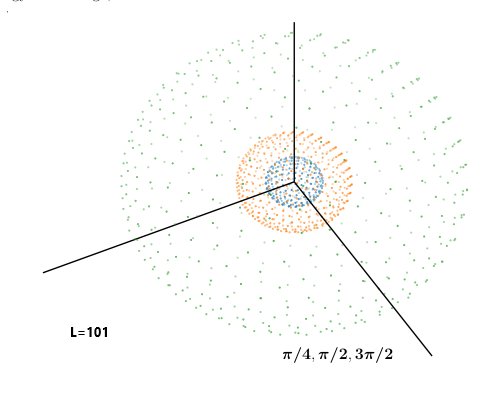
\includegraphics{fig1}}
\end{center}
\caption{The emergent $r\cdot\sin(r)$ wave cloud. \label{fig:wave-cloud} The radial interaction density of the active $s2B$ cells plotted against the radial distance $r$ from the source center (horizontal axis: integer shell radius $r=1,2,\dots$ in cells; vertical axis: normalized density of active cells on the shell).  The cell-by-cell wave amplitude follows $\sin(r)/r$, while the number of cells per spherical shell scales as $r^{2}$; their product gives the radial interaction density $r\cdot\sin(r)$ used for electromagnetic coupling.  The curve is the analytical envelope $r\sin(r)$ (arbitrary vertical scale) overlaid on the simulated shell counts; the measured match is reported in the full manuscript.}
\end{figure}


\subsection{Emergent polarization pair $(\mathrm{pol}_u,\mathrm{pol}_v)$}\label{subsec:polarization-pair}

Each active cell carries an integer pair $(u,v)$, stored as $\mathrm{pol}_u$ and $\mathrm{pol}_v$, that represents the transverse polarization in the plane tangent to the spherical wavefront.  The pair is not a geometric function of the local radius; it is derived from the \emph{broadcasted arrival stamp $b(x)$ of an elected momentum vector}.  At every turn-around of the breathing wavefront the automaton elects one direction out of its own state, a helical walker broadcasts the news of that election across the layer, and every cell converts its private arrival stamp into a polarization phase.  The mechanism has three stages---election, broadcast, and reconstruction---and uses only addition, subtraction, shift, and comparison.

\paragraph{Overview.}  The goal is to assign to each cell a direction in the plane perpendicular to an elected axis $\boldsymbol{m}$, using only integer arithmetic.  The direction is encoded as a pair $(u,v)$ lying on a circle of radius $R^2$, where $R$ is the emergent bubble radius.  The angle $\theta = \operatorname{atan2}(v,u)$ advances from $0$ to $2\pi$ as the broadcasted arrival time grows, winding a polarization helix around $\boldsymbol{m}$.  The automaton never computes $\theta$ explicitly; it computes $(u,v)$ directly from the arrival stamp using integer square roots.

\paragraph{Stage 1: Election.}  Every cell owns a predefined value $\nu\in[\,0,\,N_{I}-1\,]$---its $W$-island index, fixed once by the internal address.  At the expansion limit of the pulse (the exact tick where the wave turns from ascending to descending), every active shell cell is seeded with a \emph{payload} that combines a score (derived from $\nu$ and a global seed $s$) with the cell's linear index.  Because the index occupies the low bits, the payload order is a strict total order: ties are impossible, so the winner is unique and independent of any scan order.

Each pass lets every cell adopt the greatest payload among its six face neighbors:
\[
\mathrm{payload}(x)\;\leftarrow\;\max\bigl(\mathrm{payload}(x),\;\mathrm{payload}(x\pm e_i)\bigr),
\]
with alternating sweep directions; $2R+8$ passes guarantee full coverage of the lattice.  The true winner---the \emph{seeded} cell holding the greatest payload---is identified once, at sowing time, while the payloads are still unique; the diffusion flood merely transports the news and never redefines the winner.  The displacement from the lattice center to the winning cell becomes the momentum vector $\boldsymbol{m}$: it is rescaled to $\lvert\boldsymbol{m}\rvert=L/2$ and written onto the source-center cell of the layer.  That write is the sole dynamic initialization of $\boldsymbol{m}$; thereafter the inertia path (Sect.~\ref{subsubsec:drive pair}) treats $\boldsymbol{m}$ as immutable and only reads it to accumulate $\mathit{reloc}$ impulses.  The same elected axis drives the helical walker of Stage~2.  The next expansion limit may elect a fresh direction; nothing is prescribed at the Platonic seed, and the orientation is read off the automaton's own ledger at the instant the wave reaches its limit.

\paragraph{Stage 2: Broadcast.}  As soon as $\boldsymbol{m}$ exists, a helical walker traces the spiral arm on the pulsating bubble.  It advances one cell per tick around the cylinder whose axis is the elected direction, keeping the radial error within about one cell by purely local comparisons among its six neighbors.  The walker is an arbitrary-axis integer helix (implementation details in the source code: \texttt{spiral/spiral.c}).  During the walk, each newly computed spiral point writes one plus the current tick into its own cell of a second value lattice, reserving $b(x)=0$ for ``never reached''.

Every other tick, with alternating sweep directions, every cell inspects only its six face neighbors and copies the greatest neighbor value whenever it exceeds its own:
\[
b(x)\;\leftarrow\;\max\bigl(b(x),\;b(x\pm e_i)\bigr).
\]
No cell ever senses beyond its neighborhood, yet these monotonic values diffuse as waves that in finite time reach every cell of the lattice---global coverage achieved purely by local moves, in lockstep with the automaton tick.  Each cell therefore ends up holding the tick $b(x)$ at which the news of the elected momentum arrived.

\paragraph{Stage 3: Reconstruction.}  The arrival stamp $b(x)$ is the phase source.  A full $2\pi$ turn is encoded by $\mathrm{phase\_full}=2R^{2}$ units, where $R=L/2-2$ is the emergent bubble radius ($R$ and $\mathrm{phase\_full}$ are topological constants, Sect.~\ref{subsec:purity}).  The cell phase is read directly from the broadcasted value:
\[
\mathrm{cell\_phase}=(b(x)-1)\bmod\mathrm{phase\_full}, \qquad j=\left\lfloor\frac{\mathrm{cell\_phase}}{R}\right\rfloor .
\]
The integer $j$ ranges from $0$ to $2R-1$ and represents the position along the polarization circle.  Writing $j_{2}=j-R$ for $j\ge R$, the integer pair is reconstructed by:
\begin{align}
\text{if }j<R:\quad&u=R(R-2j),          &&v=2R\,\mathrm{isqrt}\bigl(j(R-j)\bigr),\label{eq:polu}\\
\text{if }j\ge R:\quad&u=R(2j-3R),       &&v=-2R\,\mathrm{isqrt}\bigl(j_{2}(R-j_{2})\bigr).\label{eq:polv}
\end{align}
These formulas generate an integer pair $(u,v)$ that lies on the integer lattice closest to the circle $u^{2}+v^{2}=R^{4}$ of radius $R^{2}$ (the equality is exact when the integer square root is exact, and is otherwise the closest integer approximation).  The polarization angle, defined geometrically as $\theta=\operatorname{atan2}(v,u)$, advances from $0$ to $2\pi$ as the broadcasted value grows, winding the polarization helix around the elected momentum axis.  This angle is never numerically evaluated by the automaton: it is the continuous geometric interpretation of the integer pair $(u,v)$, which encodes the direction implicitly.  No trigonometric tables, no precomputed spiral, and no per-cell fixed constants are used: the direction emerges from the tournament over the $W$-ledger, and the phase from the integer square-root relation applied to the arrival time.  Per the purity constraints (Sect.~\ref{subsec:purity}), the runtime performs no trigonometric computation whatsoever; $\operatorname{atan2}$ is introduced here only as a descriptor linking the integer pair to its emergent angular variable.

\paragraph{Fidelity of the reconstruction.}  Two quantitative statements characterize how Eqs.~\eqref{eq:polu}--\eqref{eq:polv} track the circle $u^{2}+v^{2}=R^{4}$ of radius $R^{2}$.  \emph{Radial deviation.}  The reconstructed pair never leaves the circle interior, and its deficit is purely the integer-square truncation: $u^{2}+v^{2}=R^{4}-4R^{2}\varepsilon$ with $\varepsilon=j(R-j)-\mathrm{isqrt}(j(R-j))^{2}\le R$, so the radius deviates from $R^{2}$ by at most $2R$ integer units (relative deviation $\le2/R$, vanishing wherever the integer square root is exact).  Measured maxima of the relative radial deviation decrease as $1/R$: $25.5\%$ at $R=3$, $11.6\%$ at $R=16$, $3.1\%$ at $R=64$, $0.39\%$ at $R=512$.  \emph{Angular winding.}  The angle $\theta=\operatorname{atan2}(v,u)$ winds monotonically from $0$ to $2\pi$ as the broadcasted value grows over the $2R$ steps, but the per-step spacing is not uniform: because the formula parametrizes the circle linearly in $j$ rather than in angle, the deviation from the uniform grid $\pi j/R$ saturates at about $19^{\circ}$ (maximum; mean about $12^{\circ}$) for $R\gtrsim16$, with special radii (e.g.\ $R=4$) where the sampled angles coincide exactly with the uniform grid.  Both statements are exact properties of the integer formula --- the automaton itself evaluates no trigonometric function (Sect.~\ref{subsec:purity}) --- and Table~\ref{tab:polar-fidelity} tabulates them (program \texttt{polar\_fidelity.cpp}, archived with the source).
\begin{table}[htbp]
\centering
\caption{Angular and radial fidelity of the integer polarization reconstruction (Eqs.~\eqref{eq:polu}--\eqref{eq:polv}) as a function of the emergent radius $R=R_{\mathrm{MAX}}-2$ (the tested lattice sequence $L=7,9,11,15,19,21$ corresponds to $R=1,2,3,5,7,8$).  ``Max $|\Delta\theta|$'' is the maximum over the $2R$ steps $j$ of $\lvert\mathrm{wrap}(\operatorname{atan2}(v,u)-\pi j/R)\rvert$; ``mean $|\Delta\theta|$'' its average.  ``Max rel.\ radial dev.'',\ is $\max_{j}\,(R^{2}-\sqrt{u^{2}+v^{2}})/R^{2}$, the largest deviation of the reconstructed radius from the true circle of radius $R^{2}$; it is bounded by $2/R$ and vanishes when the integer square root is exact.  Angles are post-hoc diagnostics only: the automaton performs no trigonometric computation (Sect.~\ref{subsec:purity}).  Program \texttt{polar\_fidelity.cpp}.}
\label{tab:polar-fidelity}
\renewcommand{\arraystretch}{1.2}
\begin{tabular}{|r|r|r|r|r|}
\hline
emergent radius $R$ & steps $2R$ & max $|\Delta\theta|$ (deg) & mean $|\Delta\theta|$ (deg) & max rel.\ radial dev.\\
\hline
1 & 2 & 0.000 & 0.000 & 0.000\\
2 & 4 & 0.000 & 0.000 & 0.000\\
3 & 6 & 3.435 & 2.290 & 0.255\\
5 & 10 & 17.130 & 8.438 & 0.175\\
7 & 14 & 12.946 & 8.099 & 0.131\\
8 & 16 & 11.310 & 6.641 & 0.209\\
16 & 32 & 17.306 & 9.654 & 0.116\\
32 & 64 & 17.820 & 11.096 & 0.060\\
64 & 128 & 18.686 & 11.778 & 0.031\\
\hline
\end{tabular}
\end{table}

Once these fields are present, the cyclic evolution described in Sect.~\ref{sec:light-frame} begins.  Within that structured loop particles move, interact, and display emergent physical behavior.

%%%%%%%% THE LIGHT FRAME %%%%%%%%%%
\section{The light frame}\label{sec:light-frame}
\paragraph{Era and interaction timescales.} An \emph{era} is one complete expansion of a wavefront from zero to its maximum radius followed by contraction back to zero. A light frame is an internal update sequence, not an era. Inertial interactions and the associated re-emissions are intended to occur within a few housekeeping ticks $k$, occupying only a small fraction of an era; they do not require completion of the expansion-and-contraction cycle. Dynamic initialization may require many eras before its variables stabilize. These timescales must be distinguished when interpreting numerical measurements.
The light frame (Figure \ref{fig:light_frame}) is one complete light step of the cellular automaton. It is divided into five stages: \texttt{ENCOUNTER} (interactions and pair formation), \texttt{DIFFUSION} (propagation of contact, collapse, and translation information), \texttt{RELOC} (physical displacement of source centers), \texttt{REISSUE} (re-emission of the wavefront from the new source center), and \texttt{FLOOD} (final synchronization of the three lattices). The global housekeeping counter $k$ advances synchronously in every cell, marking the current stage; the wavefront counter $t$ is local and resets to zero whenever a bubble is reissued. The separation between the common $k$ and the local $t$ is what lets the finite-state machine coordinate essentially non-local operations while keeping them intended to be strictly non-signaling: no information and no influence ever travels faster than the maximum information speed $v_{\max}$ in the idealised local rule, and causality is protected.  For the host-side scheduler of the present implementation this remains a design goal, not an established property.
Despite its name, the light frame is not a unit of light propagation: it is the period of the information clock, within which a wavefront advances exactly one lattice cell, i.e. at the maximum speed of information transmission $v_{\max}$; this rate defines the information clock rather than being an emergent prediction (the corresponding fidelity checks are reported in the full manuscript). The speed of light does not appear anywhere in the transition rule; it is emergent. An observer that measures distances and times by a round-trip convention reads the photon of Sect.~\ref{subsec:pairs}---a pair of bubbles riding the wavefront---as propagating at this speed and names it $c$. In particular, the \texttt{ENCOUNTER} stage is superluminal in coordinate terms (it compares the whole lattice along $W$ in a single sweep), but it is intended to be strictly non-signaling and cannot be manipulated by any observer; causality is thereby protected in the idealised rule, with the same host-side caveat as above.
\begin{figure}
\begin{center}
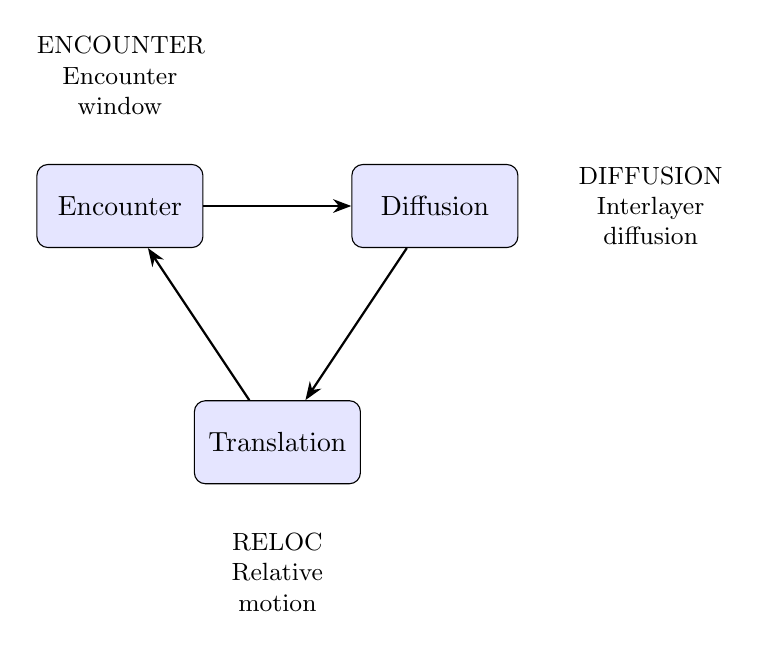
\begin{tikzpicture}[
process/.style={rectangle, rounded corners, minimum height=3em, minimum width=6em, text centered, draw=black, fill=blue!10},
arrow/.style={-Stealth, thick},
annotation/.style={text width=6em, font=\small, align=center}
]
% Define the nodes for each step (3 boxes only)
\node[process] (encounter) at (0,0) {Encounter};
\node[process] (diffusion) at (4,0) {Diffusion};
\node[process] (translation) at (2,-3) {Translation};
% Draw arrows to indicate the cyclic process (triangle shape)
\draw[arrow] (encounter) -- (diffusion);
\draw[arrow] (diffusion) -- (translation);
\draw[arrow] (translation) -- (encounter);
% Add annotations for constants
\node[annotation, above=0.5cm of encounter] (encounter-anno) {ENCOUNTER\\ Encounter window};
\node[annotation, right=0.5cm of diffusion] (diff-anno) {DIFFUSION\\ Interlayer diffusion};
\node[annotation, below=0.5cm of translation] (reloc-anno) {RELOC\\ Relative motion};
\end{tikzpicture}
\end{center}
\caption{The light frame---the period of the information clock, within which a wavefront advances exactly one lattice cell at the maximum information speed $v_{\max}$---has three stages: Encounter, Diffusion and Translation, delimited by the constants ENCOUNTER, DIFFUSION and RELOC.}
\label{fig:light_frame}
\end{figure}
\medskip\noindent\textbf{Definitions.}\label{subsec:Definitions} The frame constants of the light frame are the following:
\begin{itemize}
\item \textbf{DIAG}\\
$\lfloor\sqrt{3}\,L\rfloor$: diagonal length of the lattice; upper bound for interaction distances.
\item \textbf{RMAX}\\
$L/2$: maximum bubble radius before wrapping (the breathing-phase amplitude).
\item \textbf{ENCOUNTER}\\
$2W$: encounter window.
\item \textbf{DIFFUSION} \\
$ENCOUNTER + 2W + \lfloor\sqrt{3}(L-1)/2\rfloor + 9(L-1) + 2W$: diffusion range along $W$; also alerts all layers of an imminent collapse.
\item \textbf{RELOC}\\
$DIFFUSION + 3(L-1)$: translation phase.
\item \textbf{REISSUE}\\
$RELOC + 1$: re-emission of the wavefront from the new source center.
\item \textbf{FLOOD}\\
$REISSUE + 3(L-1)$: final synchronization of the three lattices.
\item \textbf{FRAME}\\
Same value as $FLOOD$; total duration of the light step.
\item \textbf{effective\_t}\\
Triangular breathing phase (the active-shell radius): $\mathrm{effective\_t}(t)=t\bmod L$ for $t\bmod L\le L/2$, and $L-(t\bmod L)$ otherwise.  The active-shell radius therefore advances one cell per step of the local tick $t$---i.e., per light frame---from $0$ up to the amplitude $L/2=\mathrm{RMAX}$ on the expansion branch and back to $0$ on the contraction branch; each branch lasts $L/2$ frames, so one era (one full expansion-and-contraction cycle) has period $L=2\,\mathrm{RMAX}$ in $t$ and spans $L$ light frames.  An era is distinct from a light frame and from the housekeeping tick $k$.
\end{itemize}
\subsection{Bubble, pair, singleton, and cluster} \label{subsec:pairs}
A \emph{bubble} is an expanding spherical wavefront of information organized across cells within a common layer. Spherical propagation is determined by comparing the dynamic radius $r$ to the wavefront tick $t$.
\subsubsection{Pair}
Two bubbles are overlapping if they share the same spatial coordinates and $t_1=t_2$. Overlapping bubbles can form a \emph{pair} if they have the same affinity, that is, $a_1=a_2$; the two partners share a center and phase, and their charges are complementary or matching depending on the pair's role. Pairs may remain bound to a particle as \emph{dressing} pairs or propagate freely as photons; a free pair expands outward and is gradually consumed, releasing two singletons at distinct locations.
\subsubsection{drive pair} \label{subsubsec:drive pair}
A pair can act as a \textit{drive pair}, repositioning other bubbles and providing inertia.
A drive pair is a reciprocal photon-type pair that has adopted the island's affinity $a$ and carries a non-zero transport vector $\boldsymbol{m}$, typically on the scale $L/2$. Neither a nonzero vector alone nor receiving a translation impulse makes a source a drive pair. A free pair must first acquire the particle's affinity.
Consider an island of $N$ equal-charge elements, one chief $K$ and $N-1$ delegates $D$, all sharing $a$. Its $K\times D$ and $D\times D$ contacts maintain dynamic cohesion. Without drive pairs its center of mass remains at rest in the lattice frame, although its constituents may rearrange. Bound pairs supply persistent internal propulsion through $P\times K$ and $P\times D$ contacts. A rightward resultant of their transport vectors drives a rightward mean displacement of the cohesive island. Few aligned pairs give sparse kicks and low velocity; many nearly collinear pairs give more frequent coherent kicks and higher velocity, up to the lattice transport bound. This is the proposed mechanism of inertia, not an externally imposed velocity of the aggregate.
The reference simulation algorithm resolves each unordered source contact once per light frame, counting a reciprocal pair once rather than once per half or overlapping voxel. A pair can deliver at most one unit face-step to one contacted body element, in a direction selected from $\boldsymbol{m}$; receiving that step preserves the target's $K/D$ identity. $\boldsymbol{m}$ is not a displacement of $L/2$ cells and is retained while the pair remains a drive pair. These mechanical, same-affinity contacts are not gated by the electroweak sieve.
\subsubsection{Singleton}
An unpaired bubble is called a \textit{singleton}; it is not a generic synonym for bubble.
\subsubsection{cluster}
The \textit{cluster} is a group of superposed pairs having the same affinity, same true $bB$ bits and the same (active) pBits.
\subsubsection{Specialized pairs} \label{subsec:specialized-pairs}
Certain pair combinations are not allowed to form clusters:
\begin{itemize}
\item Neutrino and antineutrino pairs possess color values $N, N$ and $\bar{N}, \bar{N}$, respectively.
\item The up quark fragments $u$ exhibit equal, nontrivial colors and a positive charge in the case of Orbis.
\item The drive pair adds to the relativistic mass of the propelled fermion.\footnote{This mirrors a Kantian view: particles do not self-move but require an external cause---here, interaction with fragments---to change their state.}
\item Pairs with fully complementary charges are \emph{gravitons}. They operate in both Orbis and Umbra,\footnote{Orbis and Umbra coexist spatially.} have fixed oscillation frequency $2$, and mediate gravity as a cross-sector, charge-sign-independent attraction; without them, Umbra matter would appear inert in Orbis. Electromagnetic static forces are instead mediated by sectorial photonic pairs (Sect.~\ref{subsec:Coulomb-interaction}). Graviton-induced gravity is detailed in the full manuscript.
\end{itemize}

\subsection{Multi frequency mechanics}\label{subsec:multi-frequency}
Dynamic initialization (the static sine/momentum masks having been removed) generates the half-wave pattern for the emergent density $r\cdot\sin(r)$, the polarization pair $(\mathrm{pol}_u,\mathrm{pol}_v)$, and the active wavefront from the integer wave equation and the elected-axis broadcast alone (Sect.~\ref{subsec:Sine} and Sect.~\ref{subsec:polarization-pair}). The radial density of active cells that pass the sieve therefore follows $r\cdot\sin(r)$ as a geometric consequence of the $\sin(r)/r$ amplitude per cell times the $r^{2}$ shell volume; no precomputed mask is required.

A photon is a single cluster with all pairs superposed. Frequency is not a continuous parameter but an integer count: a single overlapping pair at the same lattice site and wavefront radius has the fundamental even frequency $2$; a stack of $n$ such pairs has frequency $2n$. A multifrequency photon is a superposition of several such stacks (or a cluster containing populations at different even frequencies $2,4,6,\dots$). There are no continuous harmonics; the spectrum is discrete and composed only of these even-integer modes.\footnote{Laboratory and environmental photons are groups of such clusters, combined in time and space.}

Clusters are therefore intrinsically multifrequency. Each constituent pair (or stack) carries its own integer population (\texttt{pair\_count}). The automaton reads frequency as a population, not as a waveform. In the reference dynamics the count is stamped once at formation and spent by the turnaround consumption; stacks grow only where a harness seeds them, because pair formation requires two sources in the single state $S$ and cannot re-reach a formed pair. The candidate absorption rule \texttt{PAIR\_STACK\_ABSORB\_FSM} (off in the reference build) makes each detected formation register the population of identical superposed stacks on the new pair, so a stack of $n$ accumulates toward $n+1$ per encounter; dynamic stacking therefore remains part of the required mechanics below.

\begin{figure}[htbp]
\centering
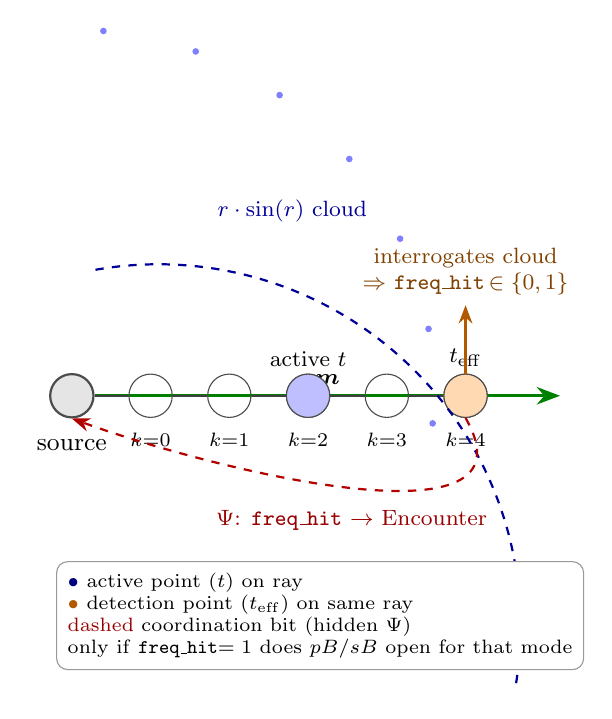
\begin{tikzpicture}[
  font=\small,
  cell/.style={circle, draw=black!70, minimum size=0.55cm, inner sep=0pt},
  activept/.style={cell, fill=blue!25},
  detectpt/.style={cell, fill=orange!30},
  centerpt/.style={cell, fill=black!10, thick},
  cloud/.style={dashed, blue!60!black},
  ray/.style={thick, black!75},
  coord/.style={-Stealth, thick, dashed, red!70!black},
  mvec/.style={-Stealth, very thick, green!50!black},
]
  % --- source centre ---
  \node[centerpt, label={[yshift=-0.15cm]below:{source}}] (C) at (0,0) {};

  % --- momentum arrow ---
  \draw[mvec] (C) -- (6.2,0) node[midway, above, black, font=\footnotesize] {$\boldsymbol{m}$};

  % --- stamped ray cells ---
  \foreach \x/\lab in {1.0/0, 2.0/1, 3.0/2, 4.0/3, 5.0/4} {
    \node[cell] (K\lab) at (\x,0) {};
    \node[font=\scriptsize, below] at (\x,-0.35) {$k{=}\lab$};
  }
  % connect ray
  \draw[ray] (C) -- (K0) -- (K1) -- (K2) -- (K3) -- (K4);

  % --- active point (t) at k=2 ---
  \node[activept] at (3.0,0) {};
  \node[font=\footnotesize, above=0.25cm] at (3.0,0) {active $t$};

  % --- detection point (t_eff) at k=4 ---
  \node[detectpt] (Det) at (5.0,0) {};
  \node[font=\footnotesize, above=0.25cm] at (5.0,0) {$t_{\mathrm{eff}}$};

  % --- cloud arc (r sin r) intersecting near detection and active ---
  \draw[cloud, thick] (0.3,1.6) arc[start angle=100, end angle=-10, radius=4.6];
  \node[font=\footnotesize, blue!60!black] at (2.8,2.35) {$r\cdot\sin(r)$ cloud};

  % dots suggesting density on the arc
  \foreach \ang in {85,70,55,40,25,10,-5} {
    \fill[blue!50] ({4.6*cos(\ang)},{4.6*sin(\ang)+0.05}) circle (1.2pt);
  }

  % --- local interrogation ---
  \draw[-Stealth, thick, orange!70!black] (Det) -- ++(0,1.15)
    node[above, font=\footnotesize, align=center, orange!50!black]
    {interrogates cloud\\$\Rightarrow$ \texttt{freq\_hit}$\,\in\{0,1\}$};

  % --- superluminal coordination back to centre ---
  \draw[coord] (Det.south) to[out=-60, in=-20]
    node[midway, below=0.15cm, font=\footnotesize, red!60!black]
    {$\Psi$: \texttt{freq\_hit} $\to$ Encounter}
    (C.south);

  % --- legend box ---
  \node[draw=black!40, rounded corners, fill=white, align=left, font=\scriptsize,
        inner sep=4pt, anchor=north west] at (-0.2,-2.1) {
    \textcolor{blue!50!black}{$\bullet$} active point ($t$) on ray\\
    \textcolor{orange!70!black}{$\bullet$} detection point ($t_{\mathrm{eff}}$) on same ray\\
    \textcolor{red!60!black}{dashed} coordination bit (hidden $\Psi$)\\
    only if \texttt{freq\_hit}$=1$ does $pB$/$sB$ open for that mode
  };
\end{tikzpicture}
\caption{Multifrequency selection on the lattice. Dynamic initialization stamps a pure-climb ray along the elected momentum $\boldsymbol{m}$. The ordinary active shell marks one cell of the ray (tick $t$). Independently, $t_{\mathrm{eff}}$ derived from \texttt{pair\_count} selects another cell of the same ray; that cell interrogates the already-propagated $r\cdot\sin(r)$ cloud and yields the binary coordination bit \texttt{freq\_hit}. The bit is written into source-centre $\Psi$ and, by the end of Encounter, gates the electromagnetic channel for that discrete mode. Different modes therefore interact at different radial phases of the same cloud.}
\label{fig:multi-frequency}
\end{figure}

\paragraph{Limitation of the present mechanism.}
The current implementation does \emph{not} yet determine the interaction point inside the $r\cdot\sin(r)$ cloud from the frequency. The active shell is set solely by the local wavefront tick of the sources ($r=\mathrm{effective\_t}(t)$), and the sieve $s2B$ is the local test
\[
\bigl((u\cdot t)\bmod S\bigr)<u,\qquad S=\mathrm{SHELL\_TARGET},
\]
gated by that same active flag. Consequently a multifrequency cluster interacts wherever its current active shell happens to lie; there is no selection of a radial phase that corresponds to a particular mode of the discrete spectrum. Electromagnetic (and magnetic) contacts therefore cannot be localized to the correct point of the cloud for a given frequency. Moreover, dynamic initialization elects the direction of the momentum vector $\boldsymbol{m}$ and installs it on the source centre, but it does \emph{not} yet materialize a straight-line sequence of cells along $\boldsymbol{m}$ on the lattice (the polarization walker produces a spiral, not a ray).

\paragraph{Required mechanics.}
Fixing multifrequency requires a linear sequence on the lattice together with a binary, frequency-conditioned trigger (Fig.~\ref{fig:multi-frequency}). The construction must remain pure (only addition, subtraction, bit shifts and comparisons of dynamic operands).

\begin{enumerate}
\item \textbf{Linear sequence along $\boldsymbol{m}$.}
  At the moment the axis is elected and $\boldsymbol{m}$ is written on the source centre, a pure-climb Bresenham walk (the climb component of the existing polarization DDA, with orbital budget set to zero) stamps successive cells along the ray with the step index $k=0,1,2,\dots,R_{\mathrm{MAX}}$. Only increments and the already-supported DDA steps are used; no multiplication or division of dynamic quantities occurs. The stamp may reuse $\mathrm{bstamp}$ or a short dedicated field. Cost is $O(R_{\mathrm{MAX}})$ and is incurred only on axis election.

\item \textbf{Effective tick from pair count.}
  The first action of Encounter for any source that carries a non-trivial $\texttt{pair\_count}$ is to form
  \[
  t_{\mathrm{eff}}=t_{\mathrm{eff}}(\texttt{pair\_count})
  \]
  by shifts and additions alone (for example $t_{\mathrm{eff}}=\texttt{pair\_count}$ or $t_{\mathrm{eff}}=\texttt{pair\_count}\ll 1$). The mapping remains a free scale choice, but it is deterministic and local to the source data.

\item \textbf{Two points on the same line.}
  On the stamped ray there are two distinguished cells:
  \begin{itemize}
  \item the \emph{active point}, corresponding to the ordinary local tick $t$ (intersection of the current active shell with the ray, or the cell whose stamp equals $t$);
  \item the \emph{detection point}, the cell whose stamp equals $t_{\mathrm{eff}}$.
  \end{itemize}
  The detection point performs a purely local interrogation of the wave cloud already present on that cell (for example $\mathit{active}\land s2B$, or a positive amplitude $u$). The outcome is a single binary result
  \[
  \texttt{freq\_hit}\in\{0,1\}.
  \]

\item \textbf{Superluminal propagation of the bit.}
  The bit $\texttt{freq\_hit}$ must become available by the end of Encounter as the effective trigger of the electromagnetic (or magnetic) channel. It is written into the draft of the source-centre cell (or reduced by a short OR-sweep strictly along the already-marked ray). Because the write targets a coordination field and does not alter readable physical fields of distant cells, the propagation is of the same character as the other non-local updates already performed inside Encounter.
\end{enumerate}

Only after $\texttt{freq\_hit}$ is true is the ordinary $pB$/$sB$ channel allowed to fire for that frequency mode. Different modes of a multifrequency cluster therefore interact at different radial phases of the same cloud; the sieve $s2B$ continues to gate local amplitude, but only after frequency has first fixed \emph{where} on the ray the gate is examined.

\paragraph{Causal coherence (superluminal non-signaling).}
The construction is examined against the formal no-signaling argument of the full manuscript. That argument partitions each cell into readable physical fields $\Phi$ (charge, affinity, radius, wave amplitudes, polarization bits, phase, active flag, local clock $t$) and hidden coordination fields $\Psi$ (housekeeping tick, $W$-ledger including $\texttt{pair\_count}$, source kind, relocation impulses, \ldots). A minimal observer reads only $\Phi$ and acts only by local rules; physical effects of any change in $\Psi$ reach other cells solely through the local six-neighbour transition and therefore at speed at most $v_{\max}$.

The bit $\texttt{freq\_hit}$ remains coherent with that partition if and only if the following conditions hold:

\begin{itemize}
\item $\texttt{freq\_hit}$ is treated as a coordination quantity ($\Psi$), never as a readable physical field ($\Phi$). A minimal observer cannot sense it directly.
\item Its only non-local write is into the draft of the source-centre cell (or another already-authorized $\Psi$ location of Encounter). Intermediate cells of the ray are not given new readable state.
\item The physical consequence of the bit---the eventual firing of the $pB$/$sB$ channel---is realized exclusively by the ordinary local transition rules (collapse, reissue, one-step motion, \ldots). From that moment onward every influence propagates at or below $v_{\max}$.
\item No admissible local intervention by an observer can modulate the bit in a controllable, spacelike fashion: $t_{\mathrm{eff}}$ is computed from data already resident at the source, and the cloud interrogation is a passive read of a field that has already been propagated by the local wave rule.
\end{itemize}

Under these restrictions the bit introduces no new species of superluminality; it re-uses the same non-signaling licence already granted to Encounter. The host-side scheduler of the present implementation inherits the same design-goal caveat already stated for all coordinated updates (see the full manuscript): the property is required of the idealised transition function, not yet established for the concrete scheduler.

The dynamic half-wave generation, the $\texttt{pair\_count}$ field with its formation and turnaround-consumption paths, the election of $\boldsymbol{m}$ and the amplitude-dependent sieve are already present in the executable (\texttt{initSim.cpp}, \texttt{simulation.cpp} \texttt{phase\_step}, \texttt{interaction.cpp}, \texttt{polarization.cpp}). Stack growth is not part of the reference dynamics: the formation rule requires both sources in the single state $S$, so the count is stamped once at formation and spent by consumption, and multifrequency populations exist only where a harness seeds them; the candidate absorption rule \texttt{PAIR\_STACK\_ABSORB\_FSM} (compiled off in the reference build) grows identical superposed stacks by one unit per encounter. The missing pieces are the pure-climb linear stamp along $\boldsymbol{m}$, the derivation of $t_{\mathrm{eff}}$, the binary detection at the stamped cell, and the coordination-only propagation of $\texttt{freq\_hit}$; all four must be introduced before electromagnetic contacts can be frequency-correct.

\subsection{Interaction principles}
The guiding principles are:
\medskip\noindent\textbf{Wavefronts clash.} The wavefronts of both bubbles must be active, i.e.\ $r_1 = \mathrm{effective\_t}(t_1)$ and $r_2 = \mathrm{effective\_t}(t_2)$, where $r_i$ is the propagated integer radius of bubble $i$ and $t_i$ is its local frame counter. This condition is assumed in all rules below.

\medskip\noindent\textbf{Aggregation and dissolution.}\label{subsec-role-of-affinity} Bubbles aggregate by sharing a common affinity; the smallest value prevails, $a_1=a_2=\min(a_1,a_2)$. On dissolution, they revert to their layer indices, $a_1=w_1$ and $a_2=w_2$. If a singleton meets a pair, the pair takes the singleton's affinity, $a_2^1=a_2^2=a_1$. The value $a=W$ marks an orphan. The idempotent $\min$ operator naturally supports an ontological model of entanglement.

\medskip\noindent\textbf{Charge conjugation.} Charge conjugation constrains interactions by requiring charge neutrality in the outcome. Electric neutrality requires a pair of opposite charges; a single bit cannot be neutral alone. Weak neutrality follows from the combination of the two weak bits in both \textit{Orbis} and \textit{Umbra}. Strong neutrality is $000$ (or $111$ for anti-neutrality); a pair with complementary color bits (e.g.\ $101$ and $010$) is also neutral. In general, interactions drive the resulting charge combination toward neutrality.

\medskip\noindent\textbf{Reciprocity.} Because only one draft can be updated at a time, the rules must later update the counterpart. This reciprocity is essential for the next subsection.
\subsection{Encounter} \label{subsec:encounter}
Encounter is the first step of the light frame (ending at $ENCOUNTER$) and contains the main interaction rules. Each site in the main lattice is compared with its partner along the $W$ dimension. This partner comparison is a rule-evaluation device that pairs lattice sites by internal address; it does not move bubbles along $W$---physical motion and merging always occur in the 3-torus (Sect.~\ref{subsec:w-islands}). For any frequency-bearing source the first actions follow Sect.~\ref{subsec:multi-frequency}: derive $t_{\mathrm{eff}}$ from \texttt{pair\_count}, interrogate the cloud at the corresponding stamped cell of the linear sequence along $\boldsymbol{m}$, and obtain the binary coordination bit \texttt{freq\_hit}. Only when that bit is set is the ordinary wave-phase $f$ and the sieve $s2B$ allowed to open the $pB$/$sB$ channel for that mode. Particles form or reform here. We postulate that the weak force only causes collapse, not limited reissues. Comparisons split into two cases: superposing or distinct bubbles.
\subsubsection{Superposing bubbles}
Two overlapping bubbles with the same wavefront tick $t_1=t_2$ can form a pair if they satisfy the following conditions:
\begin{itemize}
% Rule 1
\item
$ (q_a \oplus q_b) \land (w1_a \oplus w1_b) \land (w0_a \oplus w0_b) \land (c2_a \oplus c2_b) \land (c1_a \oplus c1_b) \land (c0_a \oplus c0_b) $
\item
% Rule 2
$ (q_a \oplus q_b) \land (w1_a = w1_b) \land (w0_a \oplus w0_b) \land (c2_a \oplus c2_b) \land (c1_a \oplus c1_b) \land (c0_a \oplus c0_b) $
\item
% TODO: add the gluon and weak boson formation rules
% Rule 3
$ ch_a = ch_b = 000000\mathrm{B} $
\item
% Rule 4
$ ch_a = ch_b = 111111\mathrm{B} $
\item
% Rule 5
$ (q_a = q_b = 0) \land (w1_a = w1_b = 0) \land (w0_a = w0_b = 1) \land (color_a = color_b) \land (color_a \neq 000\mathrm{B} \land color_a \neq 111\mathrm{B}) $
\item
% Rule 6
$ (q_a = q_b = 1) \land (w1_a = w1_b = 1) \land (w0_a = w0_b = 0) \land (color_a = color_b) \land (color_a \neq 000\mathrm{B} \land color_a \neq 111\mathrm{B}) $
\end{itemize}
To make the six rules concrete, Table~\ref{tab:charge-examples} in Appendix~\ref{app:charge-examples} lists representative bit-strings and the pairs they form (the bit order $w_{1}\,w_{0}\,q\,c_{2}\,c_{1}\,c_{0}$ and the colour code follow Table~\ref{tab:Cell-structure}).
These rules implement the formation of pairs, as defined in Sect. \ref{subsec:pairs}.
If pairs are detected, one frequency unit is registered on the pair stack (Sect.~\ref{subsec:multi-frequency}); the wave phase $f$ itself remains the triangular breathing phase of the local tick.
$s2B$ is updated as $s2B' = s2B \ \textbf{and} \ \mathit{active}$.
Notice that the pairs are formed in two steps: first, cell $a$ compares with cell $b$, and later, cell $b$ compares with cell $a$ (reciprocity).
The formation of clusters is made during this step too, also following the reciprocity principle.
Pairs are allowed to superpose if they are equal and were formed by the two first rules above.
\subsubsection{Distinct bubbles} \label{subsec:distinct}
The $w_1$ bit separates distinct-bubble interactions into same-sector ($w_1^1=w_1^2$) and inter-sector cases; we first treat same-sector interactions.
If two same-sector singletons have opposite charges and both $kB$ bits false, we have annihilation, with both bubbles being reissued from the contact point and their affinity receiving their default values. The draft $kB$ bit turns true, triggering a collapse.
Else if two singletons have the same charge, we have fermion cohesion.
One bubble is reissued from the contact point, while the other, from its active $sB$ site.
Also, they become entangled ($a_1=a_2$).
On the other hand, if the two bubbles share the same affinity, but have different charges, the bubble whose wavefront at the contact point has $pB=1$ is reissued from the contact point.
For bound $P\times K/D$ transport, the pushing pair's $\boldsymbol{m}$ selects a unit step accumulated in $\boldsymbol{\mathit{reloc}}$, as specified in Sect.~\ref{subsec:translation}; copying the full magnitude of $\boldsymbol{m}$ as a displacement is not the inertial rule. The following contact-site reissue description concerns the other interaction channels.
That is, one bubble is reissued from $\boldsymbol{x1}$, while the other from $(\boldsymbol{x_1}-\boldsymbol{x_2})\,\boldsymbol{mod}\,L$.
For color-neutral combinations there are two cases: gluon$\times$gluon and quark$\times$gluon.
In both cases, the two bubbles are reissued from the contact point and the partners colors are exchanged.
In the electroweak sector, both $\mathit{active}$ bits must be true; together with $s2B$ they determine the harmonic behavior. This sieve mechanism applies only to electroweak interactions and helps explain why the strong force is stronger.
The weak interaction occurs when the weak charges are combined to neutrality and either ($pB_1=1$, $pB_2=0$) or ($sB_1=sB_2=1$); it always triggers collapse ($kB=1$).
The electric case uses one $pB$ bit, the magnetic case one $sB$ bit. If both $pB$ bits are true (or both $sB$ bits in the magnetic case), a collapse is triggered ($kB=1$).
If only one $pB$ bit meets the other's surface, the interaction is adiabatic: no collapse occurs, but the bubbles exchange affinity and time and relocate to each other's center. The $a$ and $t$ values then spread throughout the layer.
At the initial singularity, all bubbles overlap. If two bubbles belong to different sectors and $t=RMAX/2$, they are reissued from their active $pB$ and $sB$ sites, dispersing the singularity and separating Orbis from Umbra. We call this \textit{dispersion}.
\subsubsection{Inter-sector interactions}
For inter-sector interactions, fully complementary charges lead to \textit{singularization}; otherwise the electroweak rules above apply. Singularization is the counterpart to dispersion.
The bubbles are reissued from the contact point ($pB_{curr}=\text{true}$).
%%% DIFFUSION %%%
\subsection{Diffusion, translation and collapse in one reading}\label{subsec:translation}
Three coupled tasks close the frame---diffusion, translation, and collapse handling---and are described together because they share the same coordination state.

Diffusion propagates the information needed for translation, ending at the \texttt{DIFFUSION} tick (Figure~\ref{fig:diffusion}). If any collapse bit $kB$ is set, it spreads to all bubbles sharing the same affinity, identifying every contributor to the collapsing particle.
The wave phase $f$ is not diffused: it is the local triangular breathing phase $\mathrm{effective\_t}(t)$ of each cell (Sect.~\ref{sec:light-frame}). Phases incremented by multiples of the era period interact with the wave-cloud sieve to form concentric bubbles; the active wavefront point ($t=d$) is forwarded to the Euclidean bubble through $s2B$.
At the same time, the translation vector $\mathbf{c}$ diffuses through the layer: each cell copies the first non-trivial $\mathbf{c}$ found among its neighbors. Finally, $sB$ homing increments $\boldsymbol{c}$ along any axis where a neighbor has $homB=1$, but only when the local cell has $sB=0$. By the end of diffusion, $\boldsymbol{c}$ is ready for translation.
\begin{figure}
\begin{center}
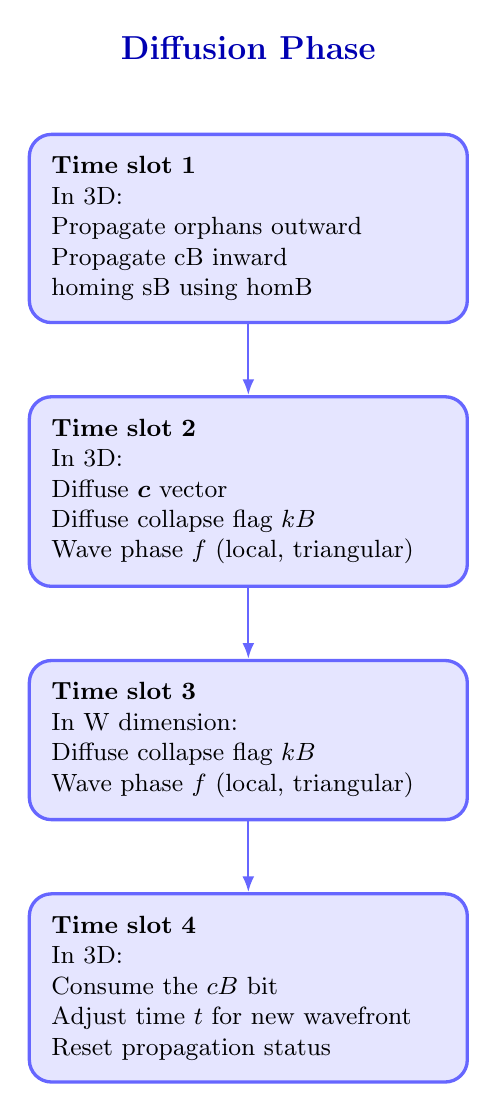
\begin{tikzpicture}[
every node/.style={font=\small, align=left},
phase/.style={rectangle, rounded corners=8pt, draw=blue!60, fill=blue!10, very thick, text width=5cm, inner sep=8pt},
arrow/.style={-{Latex[length=2mm]}, thick, blue!60}
]
% Nodes (closer spacing)
\node[phase] (t1) {
\textbf{Time slot 1}\\
In 3D:\\
Propagate orphans outward\\
Propagate cB inward\\
homing sB using homB
};
\node[phase, below=0.9cm of t1] (t2) {
\textbf{Time slot 2}\\
In 3D:\\
Diffuse $\boldsymbol{c}$ vector\\
Diffuse collapse flag $kB$\\
Wave phase $f$ (local, triangular)
};
\node[phase, below=0.9cm of t2] (t3) {
\textbf{Time slot 3}\\
In W dimension:\\
Diffuse collapse flag $kB$\\
Wave phase $f$ (local, triangular)
};
\node[phase, below=0.9cm of t3] (t4) {
\textbf{Time slot 4}\\
In 3D:\\
Consume the $cB$ bit\\
Adjust time $t$ for new wavefront\\
Reset propagation status
};
% Shorter arrows
\draw[arrow] (t1.south) -- ++(0,-0.25) -> (t2.north);
\draw[arrow] (t2.south) -- ++(0,-0.25) -> (t3.north);
\draw[arrow] (t3.south) -- ++(0,-0.25) -> (t4.north);
% Title
\node[above=0.8cm of t1, font=\bfseries\large, blue!70!black] {Diffusion Phase};
\end{tikzpicture}
\end{center}
\caption{The Diffusion phase is composed of several time slots. It spreads all information necessary for translation.}
\label{fig:diffusion}
\end{figure}
%%% Translation %%%
\medskip\noindent\textbf{Translation.} This part of the light step addresses bubble translation itself, building on the diffusion step.
It ends at the RELOC tick. Bubbles shift in specific directions (north, west, down) until they have completed their translation process, including the inertial transport mechanism.
The example rule is: if $\textbf{c}_x^{north}>0$, copy the content of the neighbor cell to the draft cell and decrement $\textbf{c}_x$ at the draft cell.
Since wavefront propagation is guided by the dynamic radius $r$ propagated from the source cell, when a bubble is re-emitted due to interaction with other bubbles, all pertinent cell information must be shifted, or relocated, to the new position determined by the variable $\textbf{c}$.
This ensures that the bubbles are relatively displaced from each other.
The final operation sets $t=0$ at the center cell of the relocated pattern.
Translation is the main consequence of an interaction.
Bubbles are re-emitted either immediately after an interaction or through wrapping.
When the bubble is reissued, the previous wavefront continues to propagate until it fades through wrapping.
In this state, the bubble is referred to as an \textit{orphan}, meaning it has affinity disabled but is still capable of non-collapsing interactions.
In this case, $a=W$ for the outer cells, set during the translation step.
To complete, the diffusion of the time variable $t$ occurs here at the last tick: When a cell has a neighboring cell with a lower $t$ value, it updates its own $t$ variable to match the lower value.
With this rule, the relocated bubble is capable of expanding again.
This timing is crucial to avoid the 'clean diamond' pattern with the new values overrunning the orphaned data.
When the translation is complete, bubble variables are prepared for the next cycle.
If the time frame completes, the $k$ counter resets to zero, preparing the system for the next iteration.
At the conclusion of the process, all $\boldsymbol{c}$ vectors will have a null value.
For internal inertial transport, source contacts are gathered during the encounter window and resolved at the end of the light frame. The numerical experiments use the following operational choices to evaluate the proposed transport mechanism. Reciprocal $K\times D$ and $D\times D$ face-steps reduce separations greater than one cell without changing the sum of body positions. Each body element can move at most once per frame. Each reciprocal drive pair pair can push at most one contacted body element; among eligible contacts it prefers the rear element along $\boldsymbol{m}$, with a rotating address tie-break. An integer DDA distributes successive face-steps in proportion to the absolute components of $\boldsymbol{m}$, retaining their signs. Zero-radius phases have no extended propelling surface. Both halves of the bound pair recycle by the same bounded face-step toward the contacted constituent. These are reference transport rules to test the proposed mechanism, not a derivation of Newtonian mechanics or rotational invariance.
The resulting unit step, rather than the full vector $\boldsymbol{m}$, enters $\boldsymbol{\mathit{reloc}}$. At the frame boundary, \texttt{applyMomentum} translates the bubble's layer state periodically, consumes the step and preserves its charge, affinity, source kind, pair identity, clock and transport vector. Translating the distance field together with its source avoids leaving a false source or stale distance minima. The source transaction commits after the voxel sweep so later cells cannot overwrite previously registered contacts or source changes. The partner rotation selects a $W$ identity; active flags are read at the current physical instant rather than from the preceding frame's shell.
The simulation algorithm uses globally coordinated source snapshots, contact arbitration, and layer translations. A strictly local cellular realization of that coordination remains to be established; the mechanical tests below validate the reference algorithm, not the purity constraints of Sect.~\ref{subsec:purity}. Dynamic initialization is never suspended, but election does not overwrite the direction of an already bound drive pair.
Let $N$ denote the number of equal $K/D$ body elements, excluding the drive pair dressing. For $n$ successful collinear unit kicks in a frame, with reciprocal cohesion contributing zero net displacement, the body's mean center of mass advances by
\begin{equation}
\Delta_{\mathrm{CoM}} \;=\; \frac{n}{N}
\end{equation}
cells per frame, with $n \leq N$. Oppositely directed steps enter with their signs; for general directions use $N^{-1}\sum_i\Delta\boldsymbol{x}_i$. This is a measured displacement identity, not a velocity assigned to the island or a mass law. drive pair-pair centers must be counted once each when separately measuring the dressed particle. Without propulsion, reciprocal cohesion preserves the body's center of mass. The displacements reported here are measured in cells per light frame. The housekeeping counter $k$ indexes the internal stages of that frame and is not the physical time used in these measurements.
Non-drive pair pairs behave differently: in $K \times K$ or $D \times D$ between different tribes the source centers move one light-step away from each other, exchanging momentum through $\boldsymbol{\mathit{reloc}}$.
An unbound pair may acquire an island's affinity through an admissible encounter. Subsequent same-affinity contacts provide propulsion; a pair of a different affinity cannot act as that island's internal drive pair. Receiving a displacement never promotes a $K/D$ source to $P$.
\medskip\noindent\textbf{Annihilation and collapse.} Annihilation and light-matter collapse both occur during the encounter stage. In annihilation, the affinity reverts to its default value $a=w$, and the resulting bubbles become raw material for new particles.
This ontological collapse introduces an arrow of time at the fundamental level, reinforcing the second law of thermodynamics and pushing Poincar\'{e} recurrence far into the future (Sect.~\ref{sec-undecidability}).
\paragraph{Reversibility.} Because Fredkin and Margolus are cited as bases (Sect.~\ref{sec:related-work}), the reversibility status should be stated explicitly.  The transition is \emph{not} injective: (i) the $s2B$ sieve discards information (the gate result is a single bit derived from a product modulo $S$); (ii) collapse sets $kB$ and reverts affinity to its default, and reissue resets the local clock $t$; (iii) relocation moves source centers and the flood stage synchronizes the three lattices by overwrite.  Each of these steps is many-to-one, so the map from one light frame to the next is not reversible, and no inverse step is defined.  This is a deliberate difference from Fredkin's reversible-computation programme: the model is a dissipative deterministic automaton with an explicit arrow of time (see above), and it is not a candidate for Landauer-free computation.  The claim is that the irreversible steps are confined to the hidden coordination fields and to the aggregate bookkeeping, so that the \emph{physical} (readable) evolution keeps its local, causal character; reversibility of the whole map is neither assumed nor required.
\subsection{Main lattice updating and partner refresh} \label{subsec:updating}
At the end of each $k$ tick, the draft lattice is transferred to main. If $k$ lies inside the $ENCOUNTER$ window, draft is first shifted along $W$ to enable encounter. This shift is a cyclic permutation of internal addresses for evaluation, not propagation of bubbles along an extra spatial axis---all physical motion remains confined to the 3-torus (Sect.~\ref{subsec:w-islands}). The partner lattice is then refreshed from main so the next encounter can compare main and partner along $W$; it copies the wave phase and active flag, $f_i^{partner}=f_i^{main}$ and $\mathit{active}_i^{partner}=\mathit{active}_i^{main}$.
\begin{figure}[ht]
\centering
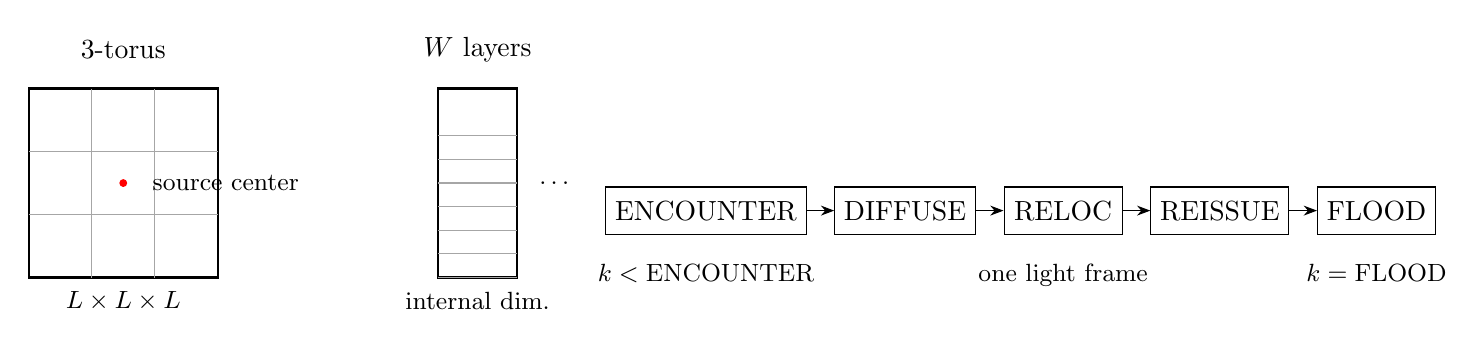
\begin{tikzpicture}[node distance=1.1cm, >=Stealth]
% --- 3-torus ---
\draw[thick] (0,0) rectangle (2.4,2.4);
\draw[gray!70] (0,0.8) -- (2.4,0.8);
\draw[gray!70] (0,1.6) -- (2.4,1.6);
\draw[gray!70] (0.8,0) -- (0.8,2.4);
\draw[gray!70] (1.6,0) -- (1.6,2.4);
\node at (1.2,2.9) {3-torus};
\node[font=\small] at (1.2,-0.3) {$L\times L\times L$};
\filldraw[red] (1.2,1.2) circle (1.2pt);
\node[font=\small, right] at (1.45,1.2) {source center};
% --- W stack ---
\begin{scope}[xshift=5.2cm]
\draw[thick] (0,0) rectangle (1.0,2.4);
\foreach \i in {0,1,2,3,4,5,6} {
\draw[gray!70] (0, 0.3*\i+0.0) -- (1.0, 0.3*\i+0.0);
}
\node at (0.5,2.9) {$W$ layers};
\node[font=\small] at (0.5,-0.3) {internal dim.};
\node[font=\small] at (1.5,1.2) {$\dots$};
\end{scope}
% --- light-frame pipeline ---
\begin{scope}[xshift=8.6cm, yshift=0.85cm]
\node[draw, rectangle, minimum width=1.5cm, minimum height=0.6cm] (c1) {ENCOUNTER};
\node[draw, rectangle, minimum width=1.5cm, minimum height=0.6cm, right=0.35cm of c1] (c2) {DIFFUSE};
\node[draw, rectangle, minimum width=1.5cm, minimum height=0.6cm, right=0.35cm of c2] (c3) {RELOC};
\node[draw, rectangle, minimum width=1.5cm, minimum height=0.6cm, right=0.35cm of c3] (c4) {REISSUE};
\node[draw, rectangle, minimum width=1.5cm, minimum height=0.6cm, right=0.35cm of c4] (c5) {FLOOD};
\draw[->] (c1) -- (c2);
\draw[->] (c2) -- (c3);
\draw[->] (c3) -- (c4);
\draw[->] (c4) -- (c5);
\node[font=\small, below=0.25cm of c1] {$k<\mathrm{ENCOUNTER}$};
\node[font=\small, below=0.25cm of c3] {one light frame};
\node[font=\small, below=0.25cm of c5] {$k=\mathrm{FLOOD}$};
\end{scope}
\end{tikzpicture}
\caption{Model architecture. \label{fig:architecture} Left: the $L\times L\times L$ 3-torus (spatial fabric), with one source center per layer emitting a spherical wavefront.  Middle: the internal dimension of $W$ layers; each layer carries one bubble and the layers are compared by the encounter stage.  Right: the light-frame pipeline of the finite-state machine---\textsc{Encounter} (interaction rules), diffusion of affinity and flags, relocation of sources, reissue, and flood---executed in $\mathrm{FRAME}$ housekeeping ticks $k$; the wavefront advances exactly one cell per tick, at the maximum information speed $v_{\max}$.}
\end{figure}
\subsection{Algorithmic summary of one light frame}\label{subsec:algorithm}
For reproducibility, Algorithms~\ref{alg:lightframe}--\ref{alg:cluster} give a self-contained account of one complete light frame: Algorithm~\ref{alg:lightframe} is the frame driver (incremental distance field, integer wave update, the six interaction stages, the charge-conjugation hook, momentum and lattice swap), and Algorithms~\ref{alg:pair}--\ref{alg:cluster} give the interaction rules invoked by the \textsc{Encounter} stage.  Together they define the full transition function; the repository (Ref.~\cite{af_neto}, \texttt{simulation.cpp}, \texttt{interaction.cpp}) is not needed to reproduce the dynamics.  The notation follows Table~\ref{tab:Cell-structure}: a charge word is written $w_{1}\,w_{0}\,q\,c_{2}\,c_{1}\,c_{0}$ (most significant first), $c_{2}c_{1}c_{0}$ is the color, $000\mathrm{B}=N$ and $111\mathrm{B}=\bar{N}$, and $\overline{ca}$ denotes the six-bit complement of the charge word $ca$.  Subscripts $a$ and $b$ label the two interacting bubbles, so $q_a$ is bit $q$ of bubble $a$, $w_{1,a}$ bit $w_{1}$ of bubble $a$, and so on.
\begin{algorithm}[ht]
\caption{One complete light frame (the full per-cell transition function, one synchronous $k$-tick).}
\label{alg:lightframe}
\begin{algorithmic}[1]
\Require $L$, $W=3L^{2}$, $\mathrm{RMAX}=L/2$, and the stage bounds
$\mathrm{ENCOUNTER}<\mathrm{GSLOT\_Z}<\mathrm{DIFFUSION}<\mathrm{RELOC}<\mathrm{REISSUE}<\mathrm{FLOOD}=\mathrm{FRAME}$ (Sect.~\ref{subsec:Definitions});
the housekeeping tick $k$, the wavefront tick $t$, and the wave phase $f=\mathrm{effective\_t}(t)$ are the cell fields of Table~\ref{tab:Cell-structure}
\Ensure the three lattices advanced by one light step
\Procedure{LightFrame}{}
\State \Call{UpdatePulsatingWavefront}{} \Comment{incremental distance field: radii $r^{2},r$ from the moving source center by $\Delta{=}2a{+}1$ increments, no square roots}
\State $pulse\_tick \gets pulse\_tick + 1$
\State \Call{PhaseStep}{} \Comment{integer wave update $v \gets v + (\nabla^{2}u \gg s)$, $u \gets u + v$, damping $v \gets v - (v \gg s_{d})$, shifts $s,s_{d}$ radius-dependent; hard zero outside the sphere; $active \Leftrightarrow r=\mathrm{effective\_t}(t)$}
\State swap $lattice\_curr \leftrightarrow lattice\_draft$
\State \Call{PolarizationTick}{} \Comment{elected-momentum broadcast over the $W$-ledger; stamps arrival ticks $b(x)$}
\For{$w = 0 \ldots W{-}1$} \Comment{loop over the internal dimension}
\For{each cell $(x,y,z)$ in the 3-torus}
\State $C \gets lattice\_curr(x,y,z,w)$; $D \gets C$; $M \gets lattice\_partner(x,y,z,w)$ \Comment{$M$: the partner cell}
\If{$k < \mathrm{ENCOUNTER}$}
\State \Call{Encounter}{$C,D,M$} \Comment{interaction rules R1--R6, Algorithms~\ref{alg:pair}--\ref{alg:cluster}; source-kind (K/S/D/P) contact re-emission and momentum impulse}
\ElsIf{$k < \mathrm{GSLOT\_Z}$}
\State glider slots \Comment{reserved for the antipodal transport schedule; not exercised by the reference simulation algorithm}
\ElsIf{$k < \mathrm{DIFFUSION}$}
\State \Call{Diffuse}{$C,D$} \Comment{orphan expansion ($a \gets W$ from a full neighbor); homing $homB \to$ translation vector $\boldsymbol{c}$; $\boldsymbol{c}$ and $kB$ transport; affinity settle}
\ElsIf{$k < \mathrm{RELOC}$}
\State \Call{Relocate}{$C,D$} \Comment{consume the translation vector $\boldsymbol{c}$ along the three axes (north, west, down)}
\ElsIf{$k < \mathrm{REISSUE}$}
\State \Call{Reissue}{$C,D$} \Comment{reset $kB,homB,bB$; propagate affinity outward from $active$ cells; consume the contraction flag $cB$ (reset $t$)}
\Else
\State \Call{Flood}{$C,D$} \Comment{synchronize the light clock: $D.t \gets \min$ of the six neighbor $t$}
\EndIf
\State $D.k \gets (C.k + 1) \bmod \mathrm{FRAME}$
\If{$D.k = 0$} \Comment{a new light frame begins}
\State $D.t \gets (C.t + 1) \bmod (2\,\mathrm{RMAX})$ \Comment{island cells ($a{=}W$, $t \le \mathrm{RMAX}$) count without the modulus}
\EndIf
\EndFor
\EndFor
\State \Call{ApplyChargeConjugation}{} \Comment{matter--antimatter turnaround hook; exact no-op when the bias $\varepsilon = 0$}
\State \Call{CommitSourceTick}{} \Comment{commit source changes; on the frame boundary resolve unique internal contacts}
\State \Call{ApplyMomentum}{} \Comment{consume free photon pairs at turnaround; translate layer states by pending steps, preserving bound-pair identity and $\boldsymbol{m}$}
\State \Call{SwapLattices}{} \Comment{$\mathrm{draft}\to\mathrm{curr}$; at $k=0$ refresh the partner ($M.f \gets \mathrm{effective\_t}(M.t)$); while $k<\mathrm{ENCOUNTER}$ rotate the partner $W$-slices (\textsc{RotatePartners})}
\EndProcedure
\end{algorithmic}
\end{algorithm}
\begin{algorithm}[ht]
\caption{Exact interaction rules for the six charge bits (superposing bubbles).}
\label{alg:pair}
\begin{algorithmic}[1]
\Function{CanFormPair}{$a,b$}
\State $ca \gets a.ch$; $cb \gets b.ch$
\If{$ca = 000000\mathrm{B}$ \textbf{and} $cb = 000000\mathrm{B}$} \Comment{R3: neutrino}
\State \Return \textbf{true}
\ElsIf{$ca = 111111\mathrm{B}$ \textbf{and} $cb = 111111\mathrm{B}$} \Comment{R4: antineutrino}
\State \Return \textbf{true}
\ElsIf{$\overline{ca} = cb$} \Comment{R1: graviton, all six bits complementary}
\State \Return \textbf{true}
\EndIf
\State $(q_a,w_{1,a},w_{0,a}) \gets$ decode bits of $ca$; $(q_b,w_{1,b},w_{0,b}) \gets$ decode bits of $cb$
\State $col_a \gets ca \& 111\mathrm{B}$; $col_b \gets cb \& 111\mathrm{B}$
\If{$q_a \neq q_b$ \textbf{and} $w_{1,a} = w_{1,b}$ \textbf{and} $w_{0,a} \neq w_{0,b}$ \textbf{and} $col_a \oplus col_b = 111\mathrm{B}$} \Comment{R2: gluon}
\State \Return \textbf{true}
\ElsIf{$q_a = q_b = 0$ \textbf{and} $w_{1,a} = w_{1,b} = 0$ \textbf{and} $w_{0,a} = w_{0,b} = 1$ \textbf{and} $col_a = col_b$ \textbf{and} $col_a \notin \{000,111\}\mathrm{B}$} \Comment{R5: up quark}
\State \Return \textbf{true}
\ElsIf{$q_a = q_b = 1$ \textbf{and} $w_{1,a} = w_{1,b} = 1$ \textbf{and} $w_{0,a} = w_{0,b} = 0$ \textbf{and} $col_a = col_b$ \textbf{and} $col_a \notin \{000,111\}\mathrm{B}$} \Comment{R6: up quark}
\State \Return \textbf{true}
\EndIf
\State \Return \textbf{false}
\EndFunction
\end{algorithmic}
\end{algorithm}
\begin{algorithm}[ht]
\caption{cluster formation, electric/magnetic channels, and collapse (superposing and distinct bubbles).}
\label{alg:cluster}
\begin{algorithmic}[1]
\Function{CanFormcluster}{$a,b$}
\State $ca \gets a.ch$; $cb \gets b.ch$
\If{$ca = cb = 000000\mathrm{B}$ \textbf{or} $ca = cb = 111111\mathrm{B}$} \Comment{R3/R4 never cluster}
\State \Return \textbf{false}
\ElsIf{$\overline{ca} = cb$} \Comment{R1 graviton never clusters}
\State \Return \textbf{false}
\EndIf
\State decode $(q,w_{1},w_{0})$ and $col$ of $ca,cb$ as in Algorithm~\ref{alg:pair}
\If{$q_a = q_b$ \textbf{and} $w_{1,a} = w_{1,b}$ \textbf{and} $w_{0,a} = w_{0,b}$ \textbf{and} $col_a = col_b$ \textbf{and} $col_a \notin \{000,111\}\mathrm{B}$} \Comment{R5/R6 up quark never clusters}
\State \Return \textbf{false}
\ElsIf{$a.\mathit{reloc} \neq 0$ \textbf{or} $b.\mathit{reloc} \neq 0$} \Comment{drive pair never clusters}
\State \Return \textbf{false}
\EndIf
\State \Return $w_{1,a} = w_{1,b}$ \textbf{and} $q_a \neq q_b$ \textbf{and} $w_{0,a} \neq w_{0,b}$ \textbf{and} $col_a \oplus col_b = 111\mathrm{B}$ \Comment{only the R2 geometry}
\EndFunction
\Procedure{Encounter}{$C,D,M$}
\State $samePos \gets C.x = M.x$; $sameT \gets C.t = M.t$
\If{$samePos$ \textbf{and} $sameT$ \textbf{and} \Call{CanFormPair}{$C,M$}}
\State $D.kind \gets M.kind \gets P$; $D.pair\_idx \gets M.w$; $M.pair\_idx \gets C.w$ \Comment{form a pair}
\State $D.a \gets M.a \gets$ shared affinity; \Call{ReemitAtContact}{$D,M$}; reset $t$
\If{$newCount > 1$ \textbf{and} \Call{CanFormcluster}{$C,M$} \textbf{and} $C.pB = M.pB$ \textbf{and} $C.sB = M.sB$ \textbf{and} $C.bB = M.bB$}
\State $D.bB \gets M.bB \gets \textbf{true}$ \Comment{cluster}
\EndIf
\ElsIf{$C.pB$ \textbf{or} $M.pB$ \textbf{or} $C.sB$ \textbf{or} $M.sB$} \Comment{electric/magnetic contact}
\If{$C.pB \wedge M.pB$ \textbf{or} $C.sB \wedge M.sB$} \Comment{collapse}
\State $D.kB \gets D.cB \gets \textbf{true}$ \Comment{triggers reissue}
\Else
\State \Call{AdiabaticExchange}{$C,D,M$} \Comment{exchange affinity and phase, relocate to partner center}
\EndIf
\EndIf
\EndProcedure
\end{algorithmic}
\end{algorithm}
As given in Sect.~\ref{subsec:updating}, \textsc{SwapLattices} transfers the draft to the main lattice at the end of every $k$ tick; at $k=0$ the partner is refreshed from main (so the next encounter compares main and partner along $W$), and while $k<\mathrm{ENCOUNTER}$ the partner $W$-slices are rotated by \textsc{RotatePartners} to schedule the cross-layer adjacency.
%%%%%%%% INTERACTIONS %%%%%%%%%%
\section{Interactions\label{sec:Interactions}}
Some interaction details are now clarified.
\subsection{Charge driven interactions}
\subsubsection{Static interactions}
Static long-range interactions are mediated by free pairs that ride the flux of orphans emitted by charged sources. The \emph{species} of the mediating pair distinguishes the force: sectorial photonic pairs (sensitive to the electric bit $q$ and to the polarization channel $pB$ or $sB$) mediate electromagnetism; fully complementary pairs---gravitons---mediate gravity. In both cases the kinematic skeleton is the same: an orphan from source $q_1$ meets a free pair; both are reissued at the contact; if the pair later meets $q_2$ it is reissued there, acquires $q_2$'s affinity, and may become a drive pair of $q_2$. The same process runs in reverse. What differs is which pair species is admitted and how the resulting drive-pair contacts bias the motion of the two sources.
\subsubsection{Coulomb interaction} \label{subsec:Coulomb-interaction}
The proposed Coulomb mechanism uses \emph{photonic} pairs, not gravitons. Orphan wavefronts from a charged source guide free photonic pairs toward another charged particle. A photonic pair becomes that particle's drive pair only after acquiring its affinity; subsequent internal contacts can then transport its $K/D$ constituents in the pair's $\boldsymbol{m}$ direction. The receiving constituent does not itself become a drive pair. Same-sign electric charges are conjectured to bias those contacts so that the two sources are driven apart; opposite signs, so that they are driven together. The polarization bit $pB$ opens the electric channel; the magnetic analogue uses $sB$ (next subsubsection). The current internal-transport tests do not establish the external capture rates, the charge-sign dependence, or a Coulomb distance law: the mechanism remains a candidate, not a measured effect.
\subsubsection{Static magnetic interaction}
The magnetic case uses the same photonic-pair mediation as Coulomb, but gates on $sB$ instead of $pB$, and applies to charged leptons, quarks and $W$ bosons. Because drive pairs emphasize $pB$ over $sB$, fast particles tend to acquire a component perpendicular to their direction of motion.
\subsubsection{Neutrino interactions}
Let $q_{0,1}$ be a complementary electric-bit pair. A neutrino fragment has charge content $q_{0,1}=00000B$; an antineutrino has $q_{0,1}=01111B$. (Anti)neutrino fragments interact only with (right-)left-handed particles.
\subsubsection{The up quark and down quark fragments}
The color combinations of fragment pairs are shown in Table~\ref{tab:color-combination}.
(Anti)\emph{quark} fragments have non-trivial color and are marked as $1q$ or $1\bar{q}$, (anti)neutrinos are $\nu$ and $\bar{\nu}$, gluons are $g$, and photons are $\gamma$.
Since half the gluon fragments are right-handed, they are shown as photons.
The shaded cells (same-color pairs) with both quarks carrying electric charge $q=+$ may form an \emph{up quark} fragment.
An \emph{up quark} $u$ can be any of the \emph{+R+R}, \emph{+G+G} or \emph{+B+B} pairs, while a \emph{down quark} $d$ can be any of the \emph{-R}, \emph{-G} or \emph{-B} single fragments. A proton fragment \emph{uud} has an uncompensated color, balanced dynamically by the matter and antimatter ends of gluons. Hence the \emph{electron} fragment must be $-N,-N,-N$.\footnote{This explains fractional quark charges.}
The number of up-quark fragments in each sector sets an upper limit on proton, and hence \textit{atom}, production.
\subsection{Self-interference\label{subsec:Interference}}
Space in this model retains a memory of particle trajectories, producing self-interference reminiscent of the double-slit experiment \cite{feynman-2}. The trace is encoded by the last affinity value $a$ and the most recent wave phase $f$ left in visited cells.
During encounter (Sect.~\ref{subsec:encounter}), incoming and residual bubbles are compared. If $d=t$, standard cohesion occurs; if $d=f$, only the new bubble is reissued, altering the fermion's dynamics and creating interference patterns. This temporally shifted interaction among the constituent ``bits'' of qubits provides a substrate for complex quantum behavior in a discrete framework.
\begin{table}[p]
\centering
\setlength{\tabcolsep}{2.2pt}
\renewcommand{\arraystretch}{0.95}
\resizebox{0.72\linewidth}{!}{%
\begin{tabular}{|c|c|c|c|c|c|c|c|c|}
\hline
&
\hdr{N}{000} &
\hdr{R}{001} &
\hdr{G}{010} &
\hdr{$\bar{\mathrm{B}}$}{011} &
\hdr{B}{100} &
\hdr{$\bar{\mathrm{G}}$}{101} &
\hdr{$\bar{\mathrm{R}}$}{110} &
\hdr{$\bar{\mathrm{N}}$}{111} \\
\hline
% N 000
\hdr{N}{000} &
\C{\nu} &
\Csec{1q}{1\ell} &
\Csec{1q}{1\ell} &
\Csec{1\overline{q}}{1\ell} &
\Csec{1q}{1\ell} &
\Csec{1\overline{q}}{1\ell} &
\Csec{1\overline{q}}{1\ell} &
\C{\gamma} \\
\hline
% R 001
\hdr{R}{001} &
\Csec{1\ell}{1q} &
\Cb{2q} &
\C{2q} &
\C{\gamma} &
\C{2q} &
\C{\gamma} &
\C{\gamma} &
\Csec{1\overline{\ell}}{1q} \\
\hline
% G 010
\hdr{G}{010} &
\Csec{1\ell}{1q} &
\C{2q} &
\Cb{2q} &
\C{g} &
\C{2q} &
\C{\gamma} &
\C{\gamma} &
\Csec{1\overline{\ell}}{1q} \\
\hline
% B-bar 011
\hdr{$\bar{\mathrm{B}}$}{011} &
\Csec{1\ell}{1\overline{q}} &
\C{g} &
\C{g} &
\Cy{2\overline{q}} &
\C{g} &
\C{2\overline{q}} &
\C{2\overline{q}} &
\Csec{1\overline{\ell}}{1\overline{q}} \\
\hline
% B 100
\hdr{B}{100} &
\Csec{1\ell}{1q} &
\C{2q} &
\C{2q} &
\C{g} &
\Cb{2q} &
\C{\gamma} &
\C{\gamma} &
\Csec{1\overline{\ell}}{1q} \\
\hline
% G-bar 101
\hdr{$\bar{\mathrm{G}}$}{101} &
\Csec{1\ell}{1\overline{q}} &
\C{g} &
\C{g} &
\C{2\overline{q}} &
\C{\gamma} &
\Cy{2\overline{q}} &
\C{2\overline{q}} &
\Csec{1\overline{\ell}}{1\overline{q}} \\
\hline
% R-bar 110
\hdr{$\bar{\mathrm{R}}$}{110} &
\Csec{1\ell}{1\overline{q}} &
\C{g} &
\C{g} &
\C{2\overline{q}} &
\C{\gamma} &
\C{2\overline{q}} &
\Cy{2\overline{q}} &
\Csec{1\overline{\ell}}{1\overline{q}} \\
\hline
% N-bar 111
\hdr{$\bar{\mathrm{N}}$}{111} &
\C{\gamma} &
\Csec{1q}{1\overline{\ell}} &
\Csec{1q}{1\overline{\ell}} &
\Csec{1\overline{q}}{1\overline{\ell}} &
\Csec{1q}{1\overline{\ell}} &
\Csec{1\overline{q}}{1\overline{\ell}} &
\Csec{1\overline{q}}{1\overline{\ell}} &
\C{\bar{\nu}} \\
\hline
\end{tabular}%
}
\caption{Color combination (rows $\times$ columns = the two fragment colors). \label{tab:color-combination}
Legend: $1q$ = one quark, $1\ell$ = one lepton, $2q$ = a quark pair (up quark), $\nu$ = neutrino, $\gamma$ = photon and $g$ = gluon; a bar denotes the antiparticle ($1\bar{q}$ = antiquark, $1\bar{\ell}$ = antilepton, $\bar{\nu}$ = antineutrino). Since half the gluon fragments are right handed, they are shown as photons. The shaded cells mark the same-color pairs that, with electric charge $q=+$, may form an \emph{up quark} fragment in Orbis (cyan, matter colors) and its anti-up (yellow, antimatter colors).}
\end{table}
%%%%%%%% PARTICLES %%%%%%%%%%
\section{Emergent island formation and the scaling of $W$}\label{sec:dynamic-charge-quantization}
This section expands Sect.~\ref{subsec:w-islands} and details how $W$-islands organize dynamically, and whether that dynamics selects a preferred population at all.
\subsection{Objects and identity}
A \emph{3D island} is a spatially localized collective of equal-charge constituents identified by its chief $K$. Each delegate $D$ refers to that chief through its parent identity. Affinity does not identify an island: multiple islands and their dressing may share one affinity, and affinity is not an eligibility condition for chief election. A complete \emph{particle} is a 3D island of bare charge plus a surrounding \emph{pair dressing}:
\begin{equation}
\text{particle} = \text{3D island} + \text{pair dressing}.
\end{equation}
The internal non-spatial dimension is partitioned into $N_I$ identical \emph{$W$-islands}, each containing
\begin{equation}
\ell = \frac{W}{N_I}
\end{equation}
positions. A $W$-island is not an object in physical space; it is an internal charge family. All $\ell$ copies inside one island share the same six charge bits ($q$, $w_1$, $w_0$, $c_2$, $c_1$, $c_0$), but each copy carries a distinct $pB$/$sB$ pattern. This built-in multiplicity is why identical particles are so similar, while the distinct polarizations allow the radial Hofer pattern to emerge.
Initially each internal address carries a singleton ($S$). Equal-charge singletons from different seed families may elect the same chief through encounter; neither their family index nor their affinity restricts this eligibility. Subsequent capture can therefore mix immutable $W$ addresses from different families within one spatial island. The proposed role of photon-mediated information transport is to enable further island formation and mixing over time; this process remains to be demonstrated numerically. A formed island has the form
\begin{equation}
1K + nD.
\end{equation}
In an admissible $D\times D$ encounter between equal-charge delegates, one delegate is promoted to a new chief $K$. Equality of charge is the only pair-specific eligibility condition: promotion does not require equal affinity, a common parent, a particular spin, or additional spatial separation beyond the general encounter conditions. The promoted source becomes its own chief, while the other source remains a delegate. This transition permits new island identities to arise after the initial singleton election; its presence must not be replaced by unconditional propagation of an existing chief identity.

Conversely, an admissible equal-charge $K\times K$ clash leaves one chief and demotes the other to a delegate of the surviving chief. In the reference experiment, the smaller W address survives; among several encountered chiefs, the smallest eligible address is retained. This is an explicit deterministic tie-break, not a demonstrated physical origin of symmetry breaking. Existing delegates of a demoted chief are not reassigned remotely by this transition. The propagation of their updated membership and the resulting balance between chief creation and removal remain subjects of the coagulation experiment.

Here $n$ counts delegates associated with the chief; the drive pair dressing is excluded. Whether the aggregation dynamics selects a \emph{preferred} population $1+n$---and whether such a preference is the same for every family, or varies with the lattice---is the open question this section tests. Nothing of the kind follows from complete membership of a seed family, and no value is imposed by initialization or election: the seed declares how many addresses \emph{share} a family ($\ell$), never how many of them should end up inside one island.

The chief gives the island its identity. Each bubble retains its intrinsic address $w$; its parent and auxiliary leader identity record its association with a chief. Sharing affinity alone neither joins two islands nor makes an $S$ a delegate. Counting chiefs and their delegates measures associations; spatial localization and persistence must be measured separately before those associations can be called stable islands. The seed bookkeeping identity is
\begin{equation}
W=3L^2=N_I\,\ell,
\end{equation}
which supplies no independent bound of $N_I$ on the number of dynamically formed chiefs: the measured chief counts exceed the declared number of families at both lattice sizes (by a factor $2.9$ at $L=9$ and $4.9$ at $L=15$).
\subsection{Is the island population quantized?}\label{subsec:dynamic-charge-quantization}
A 3D island is an open dynamical object: it continuously captures free $S$ bubbles and loses surface bubbles. Let $\Gamma_{\mathrm{cap}}(N)$ and $\Gamma_{\mathrm{esc}}(N)$ be the effective capture and escape rates for an island of characteristic population $N$. The size-selection hypothesis was originally stated as the condition that
\begin{align}
\Gamma_{\mathrm{cap}}(N) &> \Gamma_{\mathrm{esc}}(N) \quad \text{for small } N, \\
\Gamma_{\mathrm{cap}}(N) &< \Gamma_{\mathrm{esc}}(N) \quad \text{for large } N.
\end{align}
A stable attractor $N_*$ then appears near
\begin{equation}
\Gamma_{\mathrm{cap}}(N_*) \simeq \Gamma_{\mathrm{esc}}(N_*),
\end{equation}
without any global counter. The characteristic charge of a particle would be the statistically preferred population of this attractor, dressed by the required photon pairs.
The coordinated translation of Sect.~\ref{subsec:translation} is what prevents premature deterioration of such localized particles across scales, from a resting aggregate up to parton-level probing.  Because a kick displaces a single bubble while the mean center of mass advances only by $\Delta_{\mathrm{CoM}}=n/N$, no constituent ever outruns the affinity that recaptures it.  Identity survives every collapse-and-reissue because the intrinsic address $w$ is immutable while only the auxiliary \texttt{leader\_w} converges. Robustness is thus distributed over homeostasis ($N_*$), continuous affinity re-propagation at reissue, and conservative encounter rules --- not stored in any fragile global state.
\paragraph{Status: measured negative for a size-selecting attractor; the only population quantum found is 2 (reference) or 3 (candidate), rule-induced, not geometric.}
The rate-crossing formulation is \emph{degenerate} in this rule set: at the frozen plateau both capture and escape rates are \emph{zero} (no delegates leave a frozen island), so $\Gamma_{\mathrm{cap}}(N_*) = \Gamma_{\mathrm{esc}}(N_*) = 0$ selects $N_*$ by construction rather than by a dynamical balance. The only quantization this rule set produces therefore comes from the \emph{fixed-point structure of the membership transitions}, derived from the reference rules themselves with no partition parameter involved (\texttt{experiments/DYNAMIC\_QUANTIZATION\_DERIVATION.md}).
\begin{enumerate}
\item The membership transitions T1--T5 read only the numerical order of $w$, the charge word $ch$, the parent linkage, and the source kind; none of them reads $\ell$, $ISLAND\_SIZE$ or $W$. The partition enters only through the seed address map ($\lfloor w/\ell\rfloor$ giving the family index, \texttt{initSim.cpp}) and through the two candidate macros, which is why their outcome is a declared multiplicity rather than a derived quantum.
\item A frozen co-located state has at most one non-singleton group per charge word, and every such group has population $\le 2$. The bound follows from T2 (delegate promotion): any group of population $\ge 3$ contains two delegates of the same charge word, which meet within $W$ frames and promote one to chief, reducing group size by one. The maximum is reached, not merely satisfied: $K = W - 8$, $D = 8$ at both $L = 9$ ($235 + 8 = 243$) and $L = 15$ ($667 + 8 = 675$).
\item At $L = 9$, the canonical superposed-seed reference census (closed gate, $S = 16384$) freezes at $K = 235$, $D = 8$, $S = 0$, with maximum group population $2$ and no group at any larger population; the open-gate ($S = 64$) census gives $145$ K + $5$ D plus $93$ pair halves, also with maximum population $2$ (archived log \texttt{experiments/census\_ref\_el9\_s64/census.csv}: frames 2--4 identical at $K=145$, $D=5$, $P=93$). Both are reproduced exactly by the reference build.
\item At $L = 15$ ($W = 675$, $RMAX = 7$), the same reference dynamics yields $K = 667$, $D = 8$, with the population quantum again $2$ and no group above it, confirming the bound at a second lattice size with no candidate macro involved.
\end{enumerate}
A constructed balance rule that switches T2 off \emph{inside} one family (the candidate macro \texttt{DD\_INTRA\_ISLAND\_FIX}) changes only the population from 2 to 3, because the rule still uses T1/T3/T4/T5 across families. No rule in the repository produces a larger quantum without \emph{reading} the seed's multiplicity explicitly in its transition logic, which makes such a result axiomatic rather than emergent. The geometric-quantum hypothesis (shell, ball, and contact capacities) is separately tested and falsified in \texttt{experiments/GEOMETRIC\_QUANTUM.md}: no stable population matches any of the shell capacities $\{26, 66, 158, \dots\}$, the ball capacities $\{27, 93, 251, \dots\}$, or the contact capacity $W$; the realised population histogram over all 59 group-census files is a near-continuum from 1 to 33 with no quantisation gaps. The last positive path is closed: \emph{at $L \le 15$ the model has no population quantum at values other than the rule-induced 2, 3, or 5}.
\paragraph{Flux-harness confirmation.} The independent statistical instrument in \texttt{quantization/} tests the same attractor hypothesis from per-event fluxes $\Gamma_{\mathrm{cap}}(N)$ and $\Gamma_{\mathrm{esc}}(N)$ via OLS regression and permutation-surrogate testing (\texttt{quantize\_stdlib.py}). On the synthetic mean-reverting control the harness recovers $N^* = 30.38$, 95\% CI $[29.87, 30.91]$, surrogate $p = 0.005$ (PASS). On the six real datasets from the repository \emph{all four frozen configurations return zero escapes and are reported INCONCLUSIVE}: the reference at $L = 9$ and $L = 15$, the \texttt{EXCLUSION+DD\_INTRA\_ISLAND\_FIX} candidate, and the \texttt{ADDRESS\_TARGET\_FSM} candidate. Where turnover exists (the directional-channel candidates), the fitted slope is $b = +0.494$--$+0.495$, i.e. \emph{anti-restorative}---larger islands grow faster, so the population is driven upward rather than bounded. The flux harness thus confirms the membership-theorem verdict from an independent statistical angle: no population attractor exists in any real run in the repository at the accessible sizes.
\paragraph{Circulation $\mathbf{J}$ as a membership invariant (measured).}
After the population-attractor line closed, a separate programme asked whether a conserved circulation on the island could do work that a pile of members cannot. Define the integer spin of a group by
\[
\mathbf{J}=\sum_{\mathrm{members}}\mathbf{r}\times\mathbf{m},
\]
with \(\mathbf{r}\) the toroidal offset of a member from its chief and \(\mathbf{m}\) that member's momentum vector. The definition reads only \(w\), parent linkage, source centres and \(\boldsymbol{m}\); it contains no \(L\), no partition parameter and no \(\mathrm{ISLAND\_SIZE}\). Three pre-registered steps have been run (\texttt{experiments/J1\_SPIN.md}):
\begin{itemize}
\item \textbf{J0 (baseline).} Across every archived census in the repository (\(\sim 3200\) groups), \(\mathbf{J}=\mathbf{0}\) identically. The cause is structural: in the reference path body elements keep \(\boldsymbol{m}=\mathbf{0}\), so no circulation is generated.
\item \textbf{J1 (protection).} A candidate gate (\texttt{SPIN\_GATED\_FSM}) refuses delegate escape while the chief's \(\mathbf{J}\neq\mathbf{0}\). In a frozen-rotor tube where the only agent is the surface-escape rule, the \(J=0\) arm releases both delegates and the \(J\neq 0\) arm holds the group (\(1K+2D\), zero escapes), matching the four registered predictions exactly. Circulation is inert until a rule consults it; once consulted, it decides membership.
\item \textbf{J2 (selection).} The same circulation protects an already planted size; it does not produce a \(dN\)--\(N\) rate crossing or select \(N_*\). Steps that would test conservation of \(\mathbf{J}\), scaling with cavity radius, and mixed charge words remain open.
\end{itemize}
Thus \(\mathbf{J}\) is the first measured quantity in the project that can hold a group together without reading the seed's partition, but it is a \emph{protection} invariant, not a population quantum. It does not restore a size-selecting quantum; at most it can help keep an island that some other mechanism has already assembled.
\subsection{Origin of $W$ and FSM addressing}
The non-spatial dimension has size
\begin{equation}
W = 3L^2.
\end{equation}
The declared factorization
\begin{equation}
W = N_I\,\ell
\end{equation}
splits the ledger into $N_{I}$ charge families, each with $\ell=W/N_I$ identical copies. In a finite-state machine implementation the $W$ coordinate is therefore not a single integer accessed by modulo; it is a pair of registers, an island index in $[0,N_I)$ and a copy index in $[0,\ell)$. This preserves the model's FSM character: all addressing and state transitions remain local and involve only comparison, copying, and small counters.  Both integers are evaluated once at initialization from the declared topology; no rule derives them from the dynamics, and none of the aggregation results below depends on their particular value.
%%%%%%%% Sections 9 (Results) and 10 (Conjectures and prospects) are omitted in this variant; see the header of this file. %%%%%%%%%%
At this point, the core construction of the cellular automaton is complete.
\section{Conclusion\label{sec:Discussion}}
\subsection{Undecidability and long-term dynamics}\label{sec-undecidability}
Long-term dynamics involve Poincar\'{e} cycles. Because the CA can be Turing-equivalent, questions about recurrence versus chaos are undecidable in general \cite{wolfram1983,gacs1979}. The finite state space guarantees eventual recurrence (Pigeonhole principle), but the configuration space grows exponentially with $L$, making detection infeasible \cite{bernstein2007,toffoli1980}. Affinity further stretches the probable recurrence time: by binding bubbles into persistent particles and aligning them into long-lived 3D islands, it reduces the effective number of independently evolving configurations and channels the dynamics through organized attractors rather than allowing rapid, unstructured mixing. Black-hole fusion may then absorb exceptional configurations (`Gardens of Eden') and drive the system toward a Poincar\'{e} cycle. Undecidability limits algorithmic predictability, so analytical tools are needed for general insights.
\subsection{Falsifiability of the physical model}
A direct observation that an electron physically traverses both paths in a double-slit experiment would contradict the model. Self-interference here arises from recorded lattice traces, not from simultaneous path occupation.
\subsection{Novelty of the work}
Compared with prior work surveyed in Sect.~\ref{sec:related-work}, this model introduces four main novelties:
\begin{enumerate}
\item A non-spatial dimension $W$ that acts as a dynamic computational layer, enabling cross-layer encounter---a superluminal but strictly non-signaling and non-manipulable update mechanism that protects causality---and richer interactions than Zuse's purely spatial ``digital particles.''
\item Six charge bits per cell, giving Lie-group-like symmetries and Noether-like conservation at a programmable level.
\item Affinity, which groups bubbles into particles and encodes self-interference histories.
\item Ontological collapse events that break strict reversibility within a Poincar\'{e} cycle, matching the effective irreversibility of quantum measurement.
\end{enumerate}
The model retains a discrete lattice while capturing quantum and relativistic features; it remains exploratory and must still be validated against empirical data.
\subsection{Limitations and open problems}
For clarity, we collect here what the current implementation cannot yet do.  These are structural limitations of the code as it stands (small lattice, reference-modulus electroweak gate), not of the model idea; each is stated with the corresponding evidence in the full manuscript.
\begin{itemize}
\item \textbf{No measured bound-state properties yet.}  The in-simulation census registers no pair formation at the reference parameters ($\mathrm{pairM}=\mathrm{pairA}=0$, $\mathrm{form}=0$, $\mathrm{cluster}=0$), and the controlled two-bubble experiment yields a quantitative null result there: of $6{,}996$ overlapping cell-frame events only $18$ ($0.26\%$) pass the $s2B$ sieve and none triggers the pair branch.  The parameter sweep demonstrates that the pair branch \emph{can} fire ($\mathrm{form}>0$ for $S=4096,128,64,32$ at $L=7$ and $S=64$ at $L=9$), so the pair-formation channel is now a demonstrated mechanism in a parameter regime; the interaction phenomena it would mediate at the reference settings, and the properties of the produced pairs (binding energies, decay rates, cross-sections), remain unmeasured.  Bound states such as hadrons and atoms therefore remain conjectural; the aggregates that do persist (the $1K+nD$ islands of Sect.~\ref{sec:dynamic-charge-quantization}) are affinity-driven populations, not charge-bound composite particles.
\item \textbf{Continuum limit absent.}  The model is defined on a finite $3$-torus of side $L\le31$ with a single cell as the unit of length.  There is no procedure for taking $L\to\infty$ (or the cell size to zero), no coarse-graining scheme, and no derivation of a partial-differential or field-theory limit.  The $r\cdot\sin(r)$ wave cloud (Sect.~\ref{subsec:Sine}) is an emergent lattice pattern, not a solution of a continuum equation.
\item \textbf{No quantitative comparison with measured cross-sections.}  No scattering amplitude, cross-section, or decay rate has been computed from the automaton, and no quantitative particle-physics prediction follows from the model's rules; the only dimensionless comparison reported in this work (Appendix~\ref{sec:charge-census-appendix}) is a kinematic census ratio without predictive value.  Units are defined only up to the lattice scale $X$ (Appendix~\ref{sec:Calculation-of-X}); there is no mapping from cells-per-tick to physical velocities or energies.
\item \textbf{Small-lattice and boundary effects.}  The reported runs use $L=7$; the spherical cavity and the radial dead-zone at $r=\mathrm{RMAX}$ suppress corner artifacts by construction, but also truncate long-range phenomena.  The layer-symmetric seed makes all $75$ islands statistically identical, a configuration choice rather than a property of the dynamics.
\item \textbf{Electroweak channel dormant at the reference modulus only.}  The $s2B$ sieve admits fewer than $1\%$ of overlaps at the reference amplitudes and modulus, so weak phenomena---neutrino interactions, $W/Z$ fragments, decay chains, and the inter-sector rules of Sect.~\ref{subsec:distinct}---are not observed at the default settings; the sweep shows the channel firing at coarser moduli, so the reference dormancy is a parameter choice, not a structural impossibility.
\item \textbf{Open problems.}  (i)~Measure the properties (binding energy, lifetime, scattering behavior) of the pairs produced by the open $s2B$ channel, and study how the pair-formation rate depends on $S$, $U_0$, $L$ and the impact parameter; (ii)~define a continuum limit and derive effective equations; (iii)~turn the charge-combination census into genuine cross-section predictions with a unit mapping; (iv)~scale the lattice to test multi-particle dynamics beyond two bubbles; (v)~derive the model constants ($U_{0}$, sieve thresholds, $\mathrm{phase\_full}$) rather than setting them by hand.
\end{itemize}
These limitations delimit the scope of the present work: the manuscript reports mechanisms and exploratory observations, not a predictive physical theory.  The falsifiability discussion above should be read in this light.
\subsection{Future inclusions}
Ongoing work simulates the geometric structures that emerge from these local, multi-layered updates. Preliminary tests already show that the collective dynamics of fragments produce a continuous $r \cdot \sin(r)$ density cloud, localized wave-packets, stable spiral patterns and macroscopic rotations directly from discrete bit distributions. These observations support the conjecture that the universal fabric can bridge discrete local rules and the smooth symmetries of physical spacetime.
\subsection{Final thoughts}
The model is an economical ontological framework\footnote{Especially when contrasted with the Many-Worlds Interpretation of quantum theory \cite{everett1957}.} operating at a deep subatomic scale. Observable reality is approximate and emergent, with continuous spacetime symmetries (Lie, Lorentz, diffeomorphism, CPT, etc.) arising from the dynamics. Each particle is composed of an enormous number of bubbles---each a miniature universe---so intrinsic non-locality provides a natural substrate for superposition-like behavior and qubit analogs. The theory remains to be refined computationally and tested against experiment; whether it can become a predictive, falsifiable, \emph{bona fide} physical theory is an open question.
%%%%%%%% The Reproducibility subsection (manuscript.tex lines 1581-1594) is omitted in this variant; see the header of this file. %%%%%%%%%%

\section*{Nomenclature}
\begin{center}
\renewcommand{\arraystretch}{1.25}
\begin{tabular}{@{}p{2.8cm}p{9.2cm}p{2.8cm}@{}}
\hline
\textbf{Symbol} & \textbf{Meaning} & \textbf{Units}\\
\hline
$L$ & lattice side (odd integer, divisible by 3) & cells\\
$W$ & internal dimension size, $W=3L^{2}$ & layers\\
$X$ & cell size & m\\
$k$ & housekeeping (global) tick & dimensionless\\
$t$ & wavefront (local) tick & dimensionless\\
$f$ & wave phase, $f=\mathrm{effective\_t}(t)$ & dimensionless\\
$N_t$ & ticks per light frame & ticks\\
$v_{\max}$ & maximum information speed, $v_{\max}=X/N_t$ & cells per tick\\
$c$ & emergent speed of light (observer reading of $v_{\max}$) & m\,s$^{-1}$\\
$r$, $r^{2}$ & dynamic radius and squared radius from the source & cells, cells$^{2}$\\
$u$, $v$ & wave displacement and quadrature & dimensionless\\
$\mathrm{pol}_u$, $\mathrm{pol}_v$ & reconstructed transverse polarization pair & dimensionless\\
$pB$, $sB$ & polarization sign bits & boolean\\
$s2B$ & electroweak sieve test bit & boolean\\
$homB$, $cB$, $kB$, $bB$ & homing, contraction, collapse, cluster flags & boolean\\
$b(x)$ & broadcasted arrival stamp of the elected momentum & ticks\\
$ch$ & six-bit charge word ($w_1 w_0 q c_2 c_1 c_0$) & bits\\
$a$ & affinity (not spatial island identity) & dimensionless\\
$\boldsymbol{m}$ & momentum vector of a source ($\lvert\boldsymbol{m}\rvert=L/2$ typical; immutable under inertia) & cells\\
$\mathrm{reloc}$ & consumable translation impulse (filled by encounter, applied by \texttt{applyMomentum}) & cells\\
$C$ & source-center coordinate & cells\\
$\mathrm{kind}$ & source kind ($K$, $S$, $D$, $P$) & dimensionless\\
$S$ & electroweak sieve modulus ($\mathrm{s2b\_target}$) & dimensionless\\
$P(u,S)$ & sieve trigger probability & dimensionless\\
$D_{\mathrm{tot}}$, $d_{\mathrm{pair}}$, $d_{\mathrm{free}}$ & charge-census totals & dimensionless\\
$N^{*}$ & equilibrium W-island population & bubbles\\
$\Gamma_{\mathrm{cap}}$, $\Gamma_{\mathrm{esc}}$ & island capture and escape rates & bubbles per frame\\
$O$ & observable-universe diameter & m\\
$l_{P}$ & Planck length & m\\
$Ed$ & Eddington number (proton count) & dimensionless\\
$\mathrm{SEP}$ & initial bubble separation in the scattering runs & cells\\
\hline
\end{tabular}
\end{center}

%%%%%%%% FUNDING %%%%%%%%%%
\section*{Funding and competing interests}
\begin{verbatim}
The author declares that no funds, grants, or other support were received
during the preparation of this manuscript.
The author has no relevant financial or non-financial interests to disclose.
\end{verbatim}
\section*{Author contributions and AI disclosure}
\begin{verbatim}
During the preparation of this work, the authors used generative AI tools to
improve the readability and language, as well as to assist in debugging and
optimizing numerical algorithms. After using these tools, the authors reviewed
and edited the content as needed and take full responsibility for the content
of the publication.
\end{verbatim}
\printbibliography
\newpage{}
%%%%%%%% APPENDIX %%%%%%%%%%
\appendix
\begin{center}
{\LARGE{}Appendix}{\LARGE\par}
\par\end{center}
\section{Pair-rule charge examples}\label{app:charge-examples}
Table~\ref{tab:charge-examples} lists representative bit-strings that make
the six pair rules of Sect.~\ref{subsec:encounter} concrete (bit order
$w_{1}\,w_{0}\,q\,c_{2}\,c_{1}\,c_{0}$; colours follow
Table~\ref{tab:Cell-structure}: $N=000$, $R=001$, $G=010$, $\bar{B}=011$,
$B=100$, $\bar{G}=101$, $\bar{R}=110$, $\bar{N}=111$).
\begin{table}[h]
\centering
\caption{Representative charge bit-strings and the pairs they form under rules R1--R6.}
\label{tab:charge-examples}
\begin{tabular}{|c|c|c|l|}
\hline
Rule & bubble $a$ & bubble $b$ & pair formed\\
\hline
R1 & $011001$ & $100110$ & graviton (all six bits complementary)\\
R2 & $011001$ & $000110$ & gluon ($w_1$ equal, $q/w_0$/color complementary)\\
R3 & $000000$ & $000000$ & neutrino\\
R4 & $111111$ & $111111$ & antineutrino\\
R5 & $010001$ & $010001$ & up quark ($q{=}0$, $w_1{=}0$, $w_0{=}1$, color $R$)\\
R6 & $110001$ & $110001$ & up quark ($q{=}1$, $w_1{=}1$, $w_0{=}0$, color $R$)\\
\hline
\end{tabular}
\end{table}
\section{Calculation of X and L\label{sec:Calculation-of-X}}
Estimates for the value of $X$---the distance between neighbouring cells, i.e. the granularity of the grid---and for the lattice side $L$ (see Sect.~\ref{sec:space-and-time}) will be developed in this appendix.
Note that the calculations below are derivation-only: per the purity constraints (Sect.~\ref{subsec:purity}), real numbers serve solely as intermediaries to compute integer parameters and are never invoked inside the runtime transition rule.  The values of $X$ and $L$ obtained here are rounded to integers and used once at initialization as fixed topological data.
The empirical inputs used below---in particular the measured speed of light $c$ and the observed diameter of Eq.~\eqref{eq:obs}---are observer-measured quantities: $c$ is the emergent speed read from the fabric's fundamental constant $v_{\max}=X/N_t$. The appendix therefore calibrates the cell scale $X$ and the lattice side $L$ against observed data without altering the transition rule.  The calibration is one-way: the observed or assumed quantities (H1, H2) enter, and the free lattice parameter $L$ is solved from them; nothing in this appendix is derived by the transition rule, and the agreement with the observed diameter is a consistency check, not evidence for the model.
The diameter of the observable universe \cite{halpbern} is compared
to the diagonal of the lattice.
\begin{equation}
O=8.8\times10^{26}m=\sqrt{3}\,L\cdot X.\label{eq:obs}
\end{equation}
\subsection{The geometric (diameter) route}
Taking the cell scale to be the Planck length ($X=l_{P}=1.616199\times10^{-35}\,m$, hypothesis H1 below) fixes $L$ uniquely from Eq.~\eqref{eq:obs}:
\[
L \;=\; \frac{O}{\sqrt{3}\,l_{P}} \;\approx\; 3.1\times10^{61}.
\]
This is the only route that survives scrutiny.  The mnemonic $L\approx2^{202}\approx6\times10^{60}$ used in earlier versions of this paper is within a factor $\sim5$ of this value and is retained only as an order-of-magnitude slogan.

\subsection{The bookkeeping (content) route: a failed consistency check}
A second way to fix $L$ counts the baryon and photon content of the universe and requires one bubble per cell.  The average CMB photon frequency~\cite{archeops} is
\[
[f]=160\,GHz=1.6\times10^{11}\,Hz,
\]
which, converted to energy, gives
\[
E_{\mathrm{CMB}}=h\,[f]=1.060171224\times10^{-22}\,J.
\]
The proton rest energy in Joules is
\[
m_{p}c^{2}=1.503277592969\times10^{-10}\,J,
\]
so the number of average CMB photons energetically equivalent to a proton is
\[
n_{p}=\frac{m_{p}c^{2}}{E_{\mathrm{CMB}}}=1.4179573\times10^{12}.
\]
With the Eddington number $Ed=10^{80}$ as the proton count, the total proton contribution in photon units is
\[
n_{pT}=4\,Ed\,n_{p}=5.67183\times10^{92},
\]
to which the $n_{\gamma}=4\times10^{84}$ photons of the universe add nothing at this precision:
\[
n_{\gamma T}=n_{\gamma}+n_{pT}=5.67183\times10^{92}.
\]
A photon of frequency $[f]$ spans $n_{b}=[f]/f_{0}$ bubbles, where $f_{0}=c/(L\,X)$ is the frequency of one bubble; with the factor $2$ for the pair of bubbles that constitutes a photon (Sect.~\ref{subsec:pairs}), the total bubble content is
\[
n_{bT}=n_{b}\,n_{\gamma T}
=2\,\frac{[f]\,n_{\gamma T}\,L\,X}{c}.
\]
Requiring one bubble per cell, $n_{bT}=L^{3}$, gives
\[
L^{2}=\frac{2\,[f]\,n_{\gamma T}\,X}{c}
=\frac{8\,Ed\,m_{p}\,c\,X}{h},
\]
where the CMB frequency $[f]$ cancels (hypothesis H3 is therefore irrelevant to this route).  With $X=l_{P}$:
\[
L \;\approx\; 3.1\times10^{30}.
\]

\subsection{The discrepancy and why the bookkeeping route fails}
At $X=l_{P}$ the two routes disagree by
\[
\frac{L_{\mathrm{geo}}}{L_{\mathrm{book}}}
=\frac{O/(\sqrt{3}\,l_{P})}{\sqrt{8\,Ed\,m_{p}\,c\,l_{P}/h}}
\approx 1.0\times10^{31},
\]
i.e.\ by $\sim31$ orders of magnitude in $L$ and $\sim93$ orders in the total cell count $L^{3}$.  The reason is physical, not numerical: the bookkeeping route imposes one bubble per cell---a matter density of order the Planck density---whereas the actual baryon and photon content would occupy a fraction $\sim10^{-62}$ of the $10^{184}$ cells that the geometric route implies.  A content-based count therefore cannot fix the scale: the model has one space-geometric scale relation (Eq.~\eqref{eq:obs}), and the identification $n_{bT}=L^{3}$ is inconsistent with it by construction.  This is a negative result, reported so that the bookkeeping route is not mistaken for a competing derivation.

\subsection{Hypotheses and sensitivity}\label{subsec:appendixA-sensitivity}
The calculation above rests on five explicit hypotheses, none of which the model itself fixes:
\begin{itemize}
\item[H1] $X=l_{P}$: the cell scale is \emph{taken} to be the Planck length (an input hypothesis, not an output of the rule).
\item[H2] $O=8.8\times10^{26}$\,m: the diameter of the observable universe~\cite{halpbern}.
\item[H3] $[f]=160$\,GHz: the average CMB photon frequency~\cite{archeops}; enters only the failed bookkeeping route.
\item[H4] $m_{p}$: the proton rest mass (CODATA); enters only the failed bookkeeping route.
\item[H5] $Ed=10^{80}$: the Eddington number of protons in the universe; enters only the failed bookkeeping route.
\end{itemize}
Sensitivity of the surviving route: from $\ln L=\ln O-\ln\sqrt{3}-\ln X$ one has $\delta\ln L=\delta\ln O-\delta\ln X$; a relative change in either input propagates one-to-one into $L$.  A factor-2 uncertainty in $O$ or in the assumed cell scale $X$ changes $L$ by a factor 2, so the exponent is meaningful only to its order of magnitude: $L\sim10^{61}$.  The proton--electron ratio quoted in Appendix~\ref{sec:charge-census-appendix} carries the same status: a coincidence of scale, not a derived prediction.
%%%%%%%%%%%%%%%%%%%%%%%%%%%%%%%%%%%%%%%%%%%%%
\section{The charge-conjugation census: definitions, tables, and caveats\label{sec:charge-census-appendix}}
This appendix documents the combinatorial charge census summarized in the full manuscript.  It is \emph{not} a simulation of the automaton: no lattice is evolved here, and the numbers below are the output of hand-scripted random recombination of the six-bit charge words.  They are reported in full so that the reader can verify both the arithmetic and its limits.
\paragraph{Method.} The program \texttt{combine.c} (this work, archived with the source) combined $6\times32768=196{,}608$ charge-balanced fragments in several million random attempts, tabulating the averages and assuming only ``hydrogen atoms'' form.  Since the strong force dominates, the search used probability $0.001$ for up quarks and $0.999$ for gluons, based on the smallest possible charge set.  The search proceeded in four stages: gluons and up quarks (plus electrons, whose number depends on up quarks), then photons and neutrinos, then $W$ and $Z$ fragments, and finally anti-atoms.  A companion program \texttt{virada.c} probes the ``turnaround'' charge-inversion mechanism of the model with a $C$-breaking interaction asymmetry $\varepsilon=0.30$; it shows that a net sector imbalance can appear only when matter and antimatter interact at different rates, and that the sign of the imbalance follows the sign of $\varepsilon$.  Both programs are studies of the charge algebra, not outputs of the cellular automaton; they are kept out of the main text for exactly this reason.
\paragraph{Results.} Leftover bubbles that cannot form a pair or singleton indicate an ionized environment; inter-sector attenuation increases the photon count.  The data roughly resemble a few simple atoms plus multiple-pair photons.  Unmatched quark fragments may become mesons, virtual quarks, or contribute to dark matter ($50\%+25\%$).  Notably, the census shows no charge--conjugation preference in favor of antimatter: antimatter is scarce and balanced (antiup $2/2$; a single antielectron in Orbis, $1$ vs.\ $0$ in Umbra), while the only substantial sector imbalance, the complementary $W/Z$ pair, cancels out ($Z$: $24{,}592$ vs.\ $18{,}416$; $W$: $6{,}122$ vs.\ $12{,}294$; aggregate $30{,}714$ vs.\ $30{,}710$).  A static charge census therefore yields no net matter--antimatter excess; despite its naivety, the outcome is sensible as a toy universe in that any asymmetry would have to emerge from the dynamical contact rules rather than from charge counts alone.
Classifying the Orbis column into explicit matter and antimatter fragments (leptons and quarks with a definite electric charge), the census gives $83$ matter fragments ($42$ up $+10$ down $+31$ electrons) against $3$ antimatter fragments ($2$ antiup $+1$ antielectron; antiquarks vanish).  The matter-to-antimatter ratio for the charged species is therefore $83{:}3\approx27.7{:}1$.  This apparent dominance is, however, purely kinematic and not a net excess: the overwhelmingly dominant gluon species ($36{,}760$) and every ``pair'' entry (photons, gravitons, $W$, $Z$, neutrinos) are built from a fragment plus its complement, so their matter and antimatter content cancels by construction.  Only the small charged remainder is left unbalanced, and the only genuinely sector-imbalanced entries ($W/Z$) annul each other in aggregate.
\paragraph{The proton--electron mass ratio: a scale-of-consistency coincidence.} The proton--electron mass ratio comes out as $1187$ in both sectors, against the empirical value $\approx1836$ (CODATA~\cite{codata}): a relative deviation of $35\%$.  We deliberately do \emph{not} call this a prediction: the ratio depends on the hand-chosen combination probabilities and on the coarse counting of ``fragments'' in this appendix, so it is reported only as a scale-of-consistency coincidence, with no error bar and no claim of precision.  A prediction would require the ratio to emerge from the dynamical rules with quantified sensitivity to the input assumptions.
\begin{table}[h]
\centering
\caption{Charge combination (combinatorial study; averages over several million random attempts of 196,608 fragments).}
\label{combina}
\begin{centering}
{\small{}}%
\begin{tabular}{|l|c|r|r|l|}
\hline
\textbf{\small{}Fragment} & \textbf{\small{}Type} & \textbf{\small{}Orbis} & \textbf{Umbra} & \textbf{\small{}Obs.}\tabularnewline
\hline
\hline
{\small{}Gluon} & {\small{}Pair} & {\small{}36,760.0} & {\small{}36,760.0} & \tabularnewline
\hline
{\small{}Up quark} & {\small{}Pair} & {\small{}42.0} & {\small{}42.0} & \tabularnewline
\hline
{\small{}Down quark} & {\small{}Single} & {\small{}10.0} & {\small{}10.0} & \tabularnewline
\hline
{\small{}Electron} & {\small{}Single} & {\small{}31.0} & {\small{}31.0} & \tabularnewline
\hline
{\small{}Photon} & {\small{}Pair} & {\small{}20.0} & {\small{}20.0} & \tabularnewline
\hline
{\small{}Graviton} & {\small{}Pair} & {\small{}12.0} & {\small{}12.0} & \tabularnewline
\hline
{\small{}Z boson} & {\small{}Pair} & {\small{}24,592.0} & {\small{}18,416.0} & \tabularnewline
\hline
{\small{}W boson} & {\small{}Pair} & {\small{}6,122.0} & {\small{}12,294.0} & \tabularnewline
\hline
{\small{}Neutrino} & {\small{}Pair} & {\small{}6,082.0} & {\small{}6,082.0} & \tabularnewline
\hline
{\small{}Antiup} & {\small{}Pair} & {\small{}2.0} & {\small{}2.0} & \tabularnewline
\hline
{\small{}Antielectron} & {\small{}Single} & {\small{}1.0} & {\small{}0.0} & \tabularnewline
\hline
{\small{}Antiquark} & {\small{}Single} & {\small{}0.0} & {\small{}0.0} & \tabularnewline
\hline
{\small{}Leftover} & {\small{}Single} & {\small{}24,624.0} & {\small{}24,620.0} & {\small{}Adds to dark matter}\tabularnewline
\hline
\textbf{\small{}Total} &  & \multicolumn{2}{r|}{\textbf{\small{}196,587.0 }} & \tabularnewline
\hline
\end{tabular}{\small\par}
\par\end{centering}
\medskip{}
\end{table}

\end{document}